%\section{section} (h2)
%\subsection{subsection} (h3)
%\subsubsection{subsubsection} (h4)
%\paragraph{paragraph} (h5)
%\subparagraph{subparagraph}


%%signposting%%
\textit{Delve} is a narrative game currently in development. Its main interaction is player manipulation of objects in a 3D environment to influence character memories. Initially the research focus was on generating simulation events which could be narrativized and instantiated as metaphorical objects in a 3D environment. However, enough fruitful insights and challenges were generated by development of the narrativization system itself that it was eventually decided to reduce the scope of the project to just the narrativization system, and decouple it from the simulation. In comparison to \textit{Ice-Bound} and StoryAssembler, \textit{Delve} is system-complete but not content-complete. Thus, it affords an excellent opportunity to show how the Authorial Leverage Framework can inform design decisions before authoring has begun in earnest.

As with \textit{Ice-Bound} and StoryAssembler, we'll first detail the experience challenge we hoped to tackle. Then we'll detail related works in similar spaces. Because initial \textit{Delve} prototypes involved simulation-driven narrativization, we'll look at similar systems in Section \ref{subsec:simulation-driven-narrativization}. We'll then introduce Expressionist in Section \ref{subsec:expressionist}, J Ryan's system for surface text production which was used to generate the memory text. Last, because \textit{Delve} makes use of an ontology to connect between text production and object state in a metaphorical manner, we'll talk in Section \ref{subsec:computational-metaphor} about other works that have used similar techniques for a variety of aims.

We'll then discuss two prototypes that informed \textit{Delve}'s development, and yielded insights into simulation-driven narrativism. The first is \textit{LegendsWriter} in Section \ref{subsubsec:legendswriter}, a prototype that generates stories from \textit{Dwarf Fortress} game logs. We'll also discuss \textit{Argosy} in Section \ref{subsubsec:argosy-and-sculptural-sifting}, a game where the narrativism is leveraged as a player interaction mechanic. 

Having introduced these works, we'll be well-positioned to tackle \textit{Delve}'s system architecture in Section \ref{sec:delve-system-description}. Having detailed that, we'll then be able to talk about specific implementation details in Section \ref{subsec:delve-implementation-details}, leading to content creation in Section \ref{subsec:content-creation-for-delve}. With all this contextualized, we will in conclusion show how the application of the Authorial Leverage Framework applies to \textit{Delve}'s content challenges. In Section \ref{subsec:delve-traversability} we'll detail the Traversability challenges it poses, and in Section \ref{subsec:delve-authorability} how different design choices can be made within the constraints of the implemented systems to lessen the authorial burden for the upcoming content creation push.
%%signposting%%

\section{Experience Challenge}\label{sec:delve-experience-challenge}

\textit{Ice-Bound}'s system has no simulation. Its ``starting state" is whatever effects run on fixed symbol cards for a given level, and whatever themes the player has picked so far. This is less a simulation than a record of play so far, or initial constraints for story generation.

\textit{Emma's Journey} has some light simulation. Each level has a starting state for the blackboard, and each fragment can execute effects. One could make a simple simulation from these materials with each fragment executing some state change, though making such a low-grain simulation the focus of the system would be considered an ``abuse", and outside the primary aim of it. In \textit{Emma's Journey} it functioned much the way \textit{Ice-Bound}'s blackboard did: a simple record of which choices the player had made so far, available to be logically operated upon to filter future content. 

Peculiar to \textit{Emma's Journey}, StoryAssembler interfaced with the \textit{Gemini} game system \cite{summerville2018Gemini} and updated fragment text and choice availability based on a few variables that continuously changed while the mini-game was running, which could be considered a ``simulation" of sorts. But again, leaning heavily into that direction would also be outside the intended use of the narrative system.

But what if we had a narrative system that had simulation considerations ``baked in"? How can we incorporate the combinatoric design considerations of \textit{Ice-Bound} with the goal-driven capabilities and considerations of StoryAssembler within the context of a narrative simulation?

The system created to explore this narrative possibility space was \textit{Delve}. Two exploratory systems (\textit{LegendsWriter} and \textit{Argosy}) were made along the way to explore some of the affordances and implications of simulation-driven narrativization, one of the core areas \textit{Delve} engages with. \textit{LegendsWriter} and \textit{Argosy} are prototype systems created to narratively illustrate independently-operating simulations. These simulations generate a series of events according to their own logics, with their own set of considerations. The generated record of the events composes an intermediary data object. The narrative systems then use that data object to guide character story creation, threading the needle between the expressiveness of human-authored narrative, and the emergent state arising from the simulation. This approach is more ``bottom-up," because it is working to build narratives up from individual pieces, matching patterns from each step of the simulation.

After realizing how rich a simulation would be required to provide adequate material, we pivoted for \textit{Delve} to explore the idea of generating history through more of a ``top-down" method, where simulation steps are paired with narrative pieces, but the scope of the simulation goes from large to small. For example, the first step of the simulation is to find a general event which can encapsulate the totality of the time period being simulated, which is then subdivided into smaller and smaller sub-steps until it gets to individual timesteps. This afforded us more narrative control, without requiring fine-grained simulation from the get-go.

The desired play experience for \textit{Delve} necessitated taking that system further, however, as this process was meant to enable an interactive---not passively generated---experience. To accomplish this, Expressionist grammars \cite{ryan2016expressionist} (covered in Section \ref{subsec:expressionist}) are used to generate the surface text for character memories. These grammars, along with their semantic tags, are output as an intermediary data object. A translation system converts these tags to new values, which are consumed by a second system in order to create instantiated, interactable 3D objects. 

The ambitious intent with this was to create not only a system that could generate character histories, but also represent them symbolically via interactable objects in a 3D game, specifically through the lens of the \textit{method of loci} or ``memory palace", a visualization technique that dates back as far as Cicero \cite{Herrmann1988}. Said objects could then be manipulated by the player, and thus the ``memories" of the character in question could be modified, given the translation of the object's state change back into the narrative space, through the symbolic mapping (implementation details are expanded upon in Section \ref{subsubsec:delve-implementation-memory-palace-generation}).

This sort of experience would allow the playful exploration of the narrative possibility space of a character's memories, but through a level of symbolic and metaphoric remove. The main drive of gameplay would center around getting character memories into certain states, through a process of experimentation to determine what the metaphoric mappings were. These memory manipulations would pose ``mnemonic puzzles", where the player would need to figure out how to either restore or mould a character's past to a particular state, in order to reveal critical bits of the overarching narrative. This is similar in gameplay design to Horswill's \textit{MKULTRA} \cite{horswill_MKULTRA}, an AI-driven game which allows players to modify NPC beliefs through ``brainwashing" to accomplish level goals, such as retrieving an object the NPC wants to keep hidden.

These are \textit{Delve}'s long-term plans, but our first goal was building a system enabling such content to be created in the first place, so that the feasibility of the gameplay experience (and the authoring it required) could be explored. This goal was achieved, though authoring of content has yet to begin in earnest. Thus, this section will be focused on details from development of \textit{Delve} to the stage of ``all systems prototyped and operational", as well as talking about useful insights gained from two prototypes (\textit{LegendsWriter} and \textit{Argosy}) along the way. We will then show how applying the Authorial Leverage framework to \textit{Delve} before substantial authoring starts can help identify key forthcoming challenges, and suggest design and tool approaches to make authoring for \textit{Delve} more tractable.

\section{Related Works}\label{sec:delve-related-works}

\textit{Delve} touches on topics covered by a wide field of systems. Generally speaking, they fall into two broad categories: simulation-driven narrativization systems (relating to how it generates memories for characters), and computational metaphor systems (relating to how it represents them to the player). It also makes use of J Ryan's Expressionist system, which generates the surface text of memories, as well as provides the connective tissue between the two categories through semantic tagging.

We'll first talk about simulation-driven narrativization, which generates narratives using event logs from simulations. Then we'll talk about Expressionist, a system that leverages semantic tagging on grammar output to generate text. In the case of \textit{Delve}, the semantic tagging of simulation event text bridges us to the last step: translating it into a new form. The related work in ontologies and computational metaphor situates that translation process, by showing how previous efforts have been made in systemic content transformations through the use of such approaches.

\subsection{Simulation-driven Narrativization}
\label{subsec:simulation-driven-narrativization}

``Simulation games" is a broad categorization that encapsulates a variety of works made for many different artistic and entertainment goals. However, we are concerned here not so much with their form, but their \textit{substance}. Which is to say: their event data. Specifically, we are concerned with both how simulation games represent their interior events to the player, and also how third-party, external systems can make use of exported event logs to then construct post-facto narrativizations of what happens within the game.

Narrativization of games has a rich history rooted in both computer science and narratology. Most salient to our immediate purposes is ML Ryan's 1993 work on narrative in real time \cite{mimesis_baseball},  which provides a highly useful conceptual framework for thinking about how these processes interact. In it, she divides narrative into three aspects:

\begin{enumerate}
    \item the chronicle (the \textit{what}, enumerating events)
    \item the mimesis (the \textit{how}, transporting readers through description)
    \item the emplotment (the \textit{why}, the logic and design making events sensible)
\end{enumerate}

ML Ryan's framework is presented in the context of listening to a live broadcast of a baseball game and forming a narrative of what's happening, a task directly mappable to many systems through the years---up to recent efforts---that we will shortly enumerate.

ML Ryan also emphasizes a key distinction in her framework between \textit{real-time} and \textit{retrospective} narrative acts, and the tension between being able to substantially provide plot when future events are not known, versus the increased importance of plot to provide a \textit{reason} for the events to have been worth telling a story about. For example: we don't necessarily know whether a baseball game will hinge on a particular critical play. When the play first happens, the focus is on the chronicle, or \textit{what}, of it. We may also have an equivalent emphasis on \textit{mimesis}, to try to transport listeners to the stadium, so we hear the roar of the crowd, the crack of the bat, the cry of the umpire. But the emplotment, the \textit{why}, the significance of that particular play within the arc of the game, isn't wholly known---and won't be known!---until the game concludes.

However, a newspaper or announcer trying to entice people to view a game that has already concluded, will leverage all the persuasive powers of emplotment to promote the event as narratively engaging---perhaps employing some well-known tropes such as the big come-back, the upset of a champion, etc. That is, they will apply an \textit{interpretation} onto the chronicle of events to present a compelling \textit{why} of the game---how it fits into the narrative of a season or a particular team. And they will do this by (among other methods) choosing specific events in the chronicle to emphasize and report, and others to minimize or discard. This emphasis is most easily accomplished by levering a heightened \textit{mimesis} of the given events, to render them in more exquisite detail. ML Ryan's idea of history as an interpretive storytelling act is drawn and elaborated from White's earlier work on interpretive historiography \cite{white_1973}.

Therefore, this tension between chronicle and emplotment comes from an inability to predict the future. Even if we had perfect knowledge of all the events currently happening as they happened (a thought experiment Danto called the ``ideal chronicler" \cite{danto}) we would still be unable to make full use of whatever interpretive frameworks we can bring to bear on a situation. As an omniscient baseball announcer we may relate all manner of information, but despite our awesome hypothetical powers, what we \textit{wish} for is a specific set of events to happen next, a narratively charged pattern that can both make the events in the past have dramatic shape and sense, and forecast the potential of exciting developments in the future. We know the types of narrative we would \textit{like} to occur---for example, rooting for the underdog to upset the current champions---but it is impossible to tell whether that story will be the story of the game we are experiencing until certain events in the chronicle have happened.

To that related end, there's a rich seam of narrativization work in games centered around the creation of stories from chronicles of sports games, running the gamut from more traditional symbolic AI methodologies to machine learning-driven approaches, for both real-time and offline use cases. While the domain may be different, the system application and techniques are generalizable to the task of story generation from game simulation events.

\subsubsection{Live Commentary and Compelling Chronicles}\label{subsubsec:live-commentary-and-compelling-chronicles}

The Robot World-Cup Soccer (RoboCup) Simulation League is a virtual outgrowth of a physical robot competition of the same name, established in 1997 \cite{robocup} to provide a lively competitive environment to stimulate AI research on a variety of fronts. A rich community of AI researchers sprung up around it---initially for the multiple challenges of physical robot soccer. However, with the use of a server that provided the ability to stage virtual matches and export state data from them, a new opportunity presented itself: match commentary.

Three initial systems stand out for their sophistication, each from different labs: Rocco, Byrne, and MIKE \cite{andre2000three}.

Rocco is an expansion on a late 1980s prototype from the German Research Center for Artificial Intelligence (DFKI), used for automated descriptions of short soccer scenes. It was augmented by later work that resulted in a generic architecture used for multimedia reporting that could handle transformations from visual data to various styles of output, such as television-style reports and newspaper articles. To accomplish this, it used an ``incremental discourse planning mechanism", which would consult a library of previously coded knowledge on kicks or movement to match the input state, and at each increment of a time counter, calculate event salience. If no events were available, it would substitute random background information.

Rocco used state-driven templating for the generation of its surface text. The template library was hand-coded from 13.5 hours of televised soccer reports with metadata such that it could appropriately select them based on available time, bias, and report style. Rocco used a simple emotion model which could flag to change the pitch of its text-to-speech module, to communicate the agent's excitement level.

All three systems' output was speech, which introduced some productive constraints for their commentary creation. It forced not only a hard cut-off filter for events (a sports commentator can only speak so fast) but also by implication a \textit{saliency} issue---if the play had moved on while more was still to be said about a certain player or team's actions, the time to report it was lost.

Byrne, from Sony CSL, pushed the commentator aspect much further. In addition to speech, it also featured an animated head, which could express emotions while it relayed commentary. These emotions were controlled by the emotion-generation module, which managed a hierarchy of emotions ranging in intensity (1-10), a target or cause (a player action) and a decay function so they faded over time. The commentator also had a simple nationality character model, which would give it a team it supported, and some other simple variables to affect reaction emotions.

Again, because of the bandwidth constraints of speech, Byrne pruned its matching events by using a priority-scheduling algorithm. In addition to priority, events also had a ``birthday" (when it was added to the queue) and ``deadline" (when it would no longer be relevant) which were used to keep the collection of valid events fresh and topical.

The last system, MIKE, came out of the Electrotechnical Laboratory (ETL). It has the most sophisticated textual output, driven by six game state evaluation modules running simultaneously, operating at different levels of analysis. This might range from basic events (``Red3 collects the ball from Red4") to more high-level analysis like player performance evaluation (``Red1 is very active because, Red1 always takes good positions") and multi-agent strategy (``The Red-Team's formation is now breaking through enemy line from center").

Each commentary fragment is modeled as a proposition, and all modules put their fragments into one pool with importance scores, which gradually decay over time. The system selects the most salient proposition, passes it to the natural language generator, and then updates the currently active subject back to the system, to help adjust priorities for subsequent utterances. This system was later adapted by ETL into a navigation system for the blind, making use of these core architectures.

The domain of generative commentary extends to many other sports, such as horse racing. For example, systems like DEIRA \cite{deira} focus on the realism and emotional model of the commentator, using simple pre-conditions to trigger narration events, which are then grounded out using context-free grammars enhanced with state-driven templating.

The multi-agent architecture approach of MIKE has also inspired similar implementation in different contexts. Fielding et al \cite{embodied_agents} adapted a similar architecture to put actual reporters into the game as neutral players in an \textit{Unreal Tournament} capture the flag game, which then report back their observations to \textit{other} agents acting as ``editors", towards the goal of generating reports on the in-progress grame. This approach was later developed further by Tallyn et al to output both a live chronicle of the match (which more resembles a game log than human-like narration) and a longer narrative match summary \cite{embodied_agents}.

\subsubsection{Post-Match Summaries}\label{subsubsec:post-match-summaries}

There is a different thread of work for post-facto narrativization of sports games, more salient to our project with \textit{Delve}, as they operate on completed matches, and thus are released from the challenging (while productive) constraint of ``liveness", which not only limits processing time, but also the amount of emplotment that can be deployed, given the uncertainty of outcome.

Rhodes et al \cite{sports_freytag} took the example sports commentary themes from the aforementioned Ryan (\cite{mimesis_baseball}) and instantiated them through the lens of Freytag's five stages of dramatic structure \cite{freytag}, though the rise and fall of the action was replaced with the rising and falling emphasis of a particular theme. Rhodes used Lexicalised Tree-Adjoining Grammars (LTAGs) \cite{joshi1997tree} for surface text realization, which let him surface state information while avoiding repetition through the liberal use of random synonyms, which can be tweaked for intensity. While it would be a stretch to say it's on the level of color commentary, it is an interesting application of multi-event thematic progression tracking, through the application of a narrative formalism.

A couple years later in 2010, automated sports commentary was ``in the wild" with Statsheet, a sports commentary company which launched 345 websites to cover all the basketball teams of the NCAA Division 1 college basketball program, completing the task of generating over 15,000 game summaries a month \cite{statsheet}. This caused quite a panicked splash in the sports journalism community, especially in the medium of match reports, which in format are more akin to a chronicle to any sort of dramatically told story. The well-justified worry was that automated processes could provide the same level of summary with a breadth of game coverage that isn't easily achievable using human writers.

Concurrently, another sports writing website, BigTenNetwork, was also making use of a system called StatsMonkey \cite{statsmonkey} to generate match reports. StatsMonkey's architecture is centered around techniques sports reporters might use to describe a game, reified as 35 ``narrative angles", which were informed by Schank's concept of thematic structures. The events of the game are filtered by three central baseball statistics that allow them to calculate saliency values over multiple game events:

\begin{itemize}
    \item \textbf{win probability}: the likelihood of a team winning the game given the current game state
    \item \textbf{leverage index}: the historical likelihood a given event can alter win probability
    \item \textbf{game score}: a composite value to select the best players
\end{itemize}

In order to generate a match description, StatsMonkey determines a narrative angle prioritization, informed by these multi-event heuristics, and uses that, along with state-driven templating, to generate the natural language. While example output text is still succinct and seems to lack narrative concerns, these principles can be seen on display in the following example given by Allen et al \cite{statsmonkey}:

\begin{quote}
    Friday was a great day for Indiana’s Michael Earley. He hoisted the Indiana Hoosiers to an 11-9 victory over the Northwestern Wildcats (20-26). Earley blasted two home runs for Indiana (22-21). The senior right field went 3-for-5 in the game with four RBIs and two runs scored. Earley homered in the first and second innings.
\end{quote}

StatsMonkey in this case analyzed the game states and determined that Early was the most report-worthy aspect of this game, matching the ``narrative angle" of a single player carrying the team to victory, and appropriately prioritized the summary to feature him, pruning out reporting of other events as not salient to the given angle selected.

%%GDoc comments%%  
% Re-located to proper section
In more recent work involving video games as opposed to sports matches, \textit{Bardic} \cite{barot2017bardic} is a 2017 flagship system for the Liquid Narrative Group's \textit{Narrative for Sensemaking} project, which seeks to generate multimedia narratives from underlying structured game data. \textit{Bardic}'s target game was \textit{DOTA 2}, a popular multiplayer battle arena game \cite{dota}. Its goal was centered around providing several different modalities of gameplay narrativization, in order to convey different dynamics of the underlying gameplay data. For our purposes we are concerned chiefly with how it creates small stories from game logs, though it also provides generated video and a sophisticated visualization and querying tool.

To do this, \textit{Bardic} takes a game log from \textit{DOTA 2} which provides snapshots of game state at a rate of 30 times a second, with each game state containing all the attributes of each played character. Separately, the game log also includes a list of every action in the game (for their typical playthroughs the researchers dealt with roughly 60k game actions). That data then goes through a number of processes to translate and augment it, resulting in a formatted dataset. \textit{Bardic} uses an intermediary language called \textit{Impulse}, a logic-based language for narrative encoding \cite{eger2015impulse}. \textit{Impulse} represents data as \textbf{facts}, which are changed by \textbf{actions} over time, and which concern \textbf{actors} and \textbf{objects}.

\textit{Bardic} also contains hand-authored event pattern matching sequences, called \textbf{narrative tropes}. The version of \textit{Bardic} reported in \cite{barot2017bardic} contained four initial tropes (though the team expressed a plan to add more in the future): 

\begin{enumerate}
    \item chase fight (one character fleeing while being attacked)
    \item alpha strike (many on one)
    \item hard work montage (repeated actions to achieve a goal)
    \item failure montage (multiple actions and failing to reach a goal)
\end{enumerate}

\textit{Bardic} then takes a user-selected subset of this data, and---given a list of which valid narrative tropes to apply---uses a planner to filter events to the subset that fit that trope. Once achieved, it grounds out the event symbols (such as characters or properties) to surface text.

The output text is simple and descriptive. For example: ``Dazzle was a main-actor. He damaged Crystal Maiden for 22 damage with a poison touch. Then he moved from the Radiant Base to the Bottom Inner Radiant Tower. Next he damaged Crystal Maiden for 22 damage with the poison touch. Then he killed her because he damaged her for 22 damage with the poison touch. Next he healed Wisp for 25 damage. Then he died" \cite{barot2017bardic}.
%%GDoc comments%%  
%%GDoc comments%%
This is still an active area of inquiry, with efforts like Shah et al's work in 2019 \cite{shah} tackling commentary generation for ``Let's Play" videos of \textit{Minecraft}, using a convolutional network. However, for our purposes we are more concerned with output resembling well-formed narrative in its own right, rather than simply descriptive sequences of game events. That said, these systems and the formalizations they employ to achieve their generative goals are potentially fruitful lessons in techniques that could be applied to such a task.
%%GDoc comments%%

\subsubsection{Playthrough Retellings}\label{subsubsec:playthrough-retellings}

Other formalisms have been used to convert playthroughs of simulation games to story in a more structured way. Antoun et al \cite{antoun2015generating} tackled creating narrativizations of the high school drama simulation game \textit{Prom Week} \cite{mccoy2012prom} using story intention graphs (SIGS) \cite{elson_SIG}, a semantic narrative representation that has been applied by other researchers to other works such as TellTale's \textit{The Wolf Among Us} \cite{Murray_wolf}. While their work remained somewhat proof-of-concept, Antoun et al's approach was to automatically derive structured plot data from harvested playthroughs of the game. Unfortunately they found in the pursuit of this that, while with some effort on their part they were able to encode the features of playtraces into SIGs, the stories generated by the playthroughs lacked coherence. This potentially could have been due to a feature mismatch of the SIG specification and the underlying simulation of \textit{Prom Week}, which made translation between the two difficult. Regardless, the approach of taking a technique usually deployed to hand-encode stories for analysis, and attempt to backchain it instead to generate stories from structured data, is a compelling thread of research.

So far we've seen how third-party applications might make sense of a game, whether that be baseball, horse racing, first-person shooters, or high school social simulations. However, there are also games which generate and represent their own histories to players internally. This is also useful for us to examine, as it directly relates to surfacing simulation state in a narrative manner.

\subsubsection{Internal Representations: History as Process and Artifact}\label{subsubsec:internal-representations}

Simulations are excellent event generators. Their positioning as a cohesive world, even if fictional, means that their events suggest an authoritative history, or at least a historical chronicle. But because history is intrinsically the process of meaning-making, a simple recording of events isn't enough to relate a story. As put forward by ML Ryan and White, that requires interpretation. In our case that might mean the person reading the record, or perhaps other processes within the game.

There are some illustrative simulation games that pre-generate events to create their worlds. When a player starts a game of \textit{Caves of Qud} \cite{qud}, an indie procedural rogue-like game, the system first generates the history of the world up to that point, populating the sultans and their respective historical domains, and using that to drive other processes to formulate groups and societies, complete with rivalries and alliances. Grinblat and Bucklew, the creators, are very conscious of the choices made to create this historical narrative, and broadly categorize two different approaches to simulating history in games: history as process, and history as artifact:

\begin{quote}
    There’s a distinction to be made between history as a process and history as an artifact. The former can be conceptualized as the playing out of rules and relationships that continually produce the present. To simulate this process, we might seek to reproduce its logic. On the other hand, the latter is a constituent of the present, something we engage with through a contemporary lens and whose complexities may be obscured by that flattening of perspective. \cite{grinblat2017subverting}
\end{quote}

Viewing this from a systems design standpoint, one could say that generated history as a process directly engages with the code that produces the events in-game, and history as an artifact takes the data generated from the event simulation, and uses that in a separate system to generate a history that can either cleave tightly, or distantly, to the original events. The latter is an intriguing design space that the systems in this section engage with.

\textit{Dwarf Fortress} \cite{dwarfFortress}, a famous work within the genre of rogue-likes, could be said to be the exemplar of ``history as process." \textit{Dwarf Fortress} is a massive simulation game that has been in focused development since 2004 \cite{df_history}. The seventeen years of effort have resulted in one of the most baroque, elaborate, and intricate works of simulation in perhaps all of games as a medium.

Foregrounded by the game is its autonomous simulation of history. The first thing a player does when starting a new game is decide how big a world they want to play in, and for how long the simulation should create world history before their game starts. World generation can run from a minute or two, to the extreme case of more than a week, if all parameters are maximized. In this last case, I generated the world Opuorid with maximum settings (a large-scale world for 10,000 years of history) and after several failed attempts, lucked into a random seed that completed in just a little over ten days of constant generation.

\textit{Dwarf Fortress}'s simulation runs a gamut of processes, from simulation of physical geologic forces that form mountains and valleys, to erosion, to the propagation of plants to form biomes, to the socioeconomic forces governing the expansion of cities, complete with alliances, political intrigue, wars both military and trade, as well as a wealth of culture, including unique dance, poetry, and song. This all happens without player input, is absolutely unique each time, yet utilizes the same processes in a predictable---if staggeringly complex---manner.

Once world generation has concluded, the player is presented with three ways to interact with the game. In ``Fortress Mode", the titular and perhaps most well-known mode, the player picks an embarkment site, and begins the game with a group of dwarves. From there, they command the dwarves to complete various tasks, with the ultimate goal of creating a successful fortress. In ``Adventurer Mode", the player chooses a race and town to start in, and is instantiated into the game as a character. This mode is a bona fide rogue-like, where the player controls their character, levels up skills, has adventures, and explores the world. In the mode we are most interested in, ``Legends Mode", the events of the world simulated to date are presented to the player in a simple text interface, and they can read about historical figures, large battles, and important historical sites. They cannot impact or enact change upon the world in this mode, only read what has been generated thus far.

While there are three different modes, all three interact with the same underlying world, and the same event and entity materials generated by it. A player can play as a single character until they are a high level, retire that character at a town, start a game to form a fortress, and have their old character come to investigate the fortress once it's established. If the player then commands the dwarves to take in that adventurer and they play a pivotal role in the fortress, the player can later check in Legends Mode and see a terse chronicle of those exploits.

Similarly, a player can successfully play a fortress until it is established and mighty, retire the fortress, let time pass, start an adventurer, then find its ruins. By talking to townsfolk (or using Legends Mode) they may learn a terse description of what befell it, and piece together a narrative.

Importantly, there is no win state in \textit{Dwarf Fortress}, although one can---and undoubtedly will---lose frequently. In no matter the mode, the player continues to play until they tire of their world, and stop the game when they are satisfied. This is an intriguing positioning for a game, because it foregrounds the world as something that is largely happening---for the most part---without player intervention, and furthermore has existed without player input for many more years than their impact upon it. Before the player's very first action, there are already far more events generated by the system than the player could ever generate through their gameplay. Thus there's a sense that whatever small dramas play out in the course of their game, they take place against a large and intricate backdrop of story that makes up every town, every goblin and kobold and elf in the game.

The logics for these generated events are systemically implemented, but a good portion actually have their genesis in short stories. In an interview with GamaSutra \cite{df_history}, Tarn Adams revealed that development of which systems to simulate is driven---at least partially---by the short stories of his brother Zach. Indeed, a section of \textit{Dwarf Fortress}'s website has a listing of Zach's stories, after which is a detailed breakdown of what systemic formalizations they seem to suggest, to be added into the feature queue for further development \cite{df_stories}. A story about assassination might yield development of animals as messengers, or a relatively short story about magic may seed a staggering litany of development tasks that stretch over multiple years.

However, while \textit{Dwarf Fortress} may have as one of its goals the faithful simulation of a world that can give rise to stories such as the ones written by Zach Adams, the Legends mode for browsing the storied events has more in common with the medieval chronicle than a short story, as Boluk and LeMieux noted \cite{boluk2013dwarven}. Talking to characters in-game can yield short descriptions about historic events or figures, but ultimately the task falls to the player to flesh out these chains to fully-formed stories, usually ending with the character or fortress's untimely demise. Boluk and LeMieux term these ``Dwarven Epitaphs", ``postmortem accounts of play [that] navigate the interstices of fanfiction, fan translation, and fan archiving not only to expand the field of play beyond the boundaries of software but also to explore the intersection of making and critique" \cite{boluk2013dwarven}. These epitaphs might take the form of serial posts on forums (as with the Chronicle of Boatmurdered \cite{boatmurdered}) serial comics (such as Oilfurnace \cite{denee}), or any number of other media. The purpose of all these engagements in the liminal space between the game and the fans is to ``convert world generator to story generator and mark the dissonant registers produced between human operators and nonhuman operations." \cite{boluk2013dwarven}

What if a second set of systems was developed to do just this? As with the sports commentary systems, which seek to narrativize the processes and outcomes of the games (which the viewers have no impact or role in), what if we applied that same descriptive goal to \textit{Dwarf Fortress}? Indeed, \textit{Dwarf Fortress} is a uniquely suited testbed, as one can export its ``Legends file`` as an XML with a representation of every simulated event in the game, along with the relevant historical figures and entities (such as civilizations, armies, etc). Furthermore, through a set of Lua tools called DFHack \cite{dfHack}, modders have been able to construct tie-in programs that react to and work with \textit{Dwarf Fortress} data by reading the states of memory addresses. One such program is LegendsViewer \cite{legendsviewer}, which works with all the events generated by the game during its world generation phase, collates them to XML, and parses them into a .Net application, namely an explorable wiki. From this, it is possible to trace historical figures through their lives as they fight, change professions, marry, form empires, and die (to name but a few possibilities). Even more critically, LegendsViewer is open source, and thus easily accessible to extend and modify the work already done to provide its chronicle-like output to something more closely resembling a story.

If \textit{Dwarf Fortress} handles the logic of simulation, and those processes are fairly well known, then one should be able to craft a separate series of systems that can generate stories from those events, using the procedures and logics of the simulation to bolster their narrative connective tissue. Or, to borrow Grinblat and Bucklew's terminology, we can construct our own historical artifact, using as raw material the XML generated by the history-as-process of the game itself. This artifact could be colored by perspective and processes totally outside the scope of the original data, and still be a compelling retelling of the ``historic events" of the simulation.

J Ryan formalized this approach as ``curationist architecture" \cite[p.~232]{ryan2018curating}, which is a useful lens to view not only this project, but narrativist systems in general. This particular approach is more specifically ``feedforward" curation, in which the story that's created has no procedural hook back into the simulation. It exists independently, a sort of generative spandrel\footnote{A spandrel in evolutionary biology is a characteristic which is orphaned from the process of natural selection, yet still provides the organism with a distinguishing characteristic.} to the core procedures of the game itself. This architecture can be summarized as the components in Figure  \ref{fig:curationist-architecture-components}.

%%%%%%%% BEGIN FIGURE %%%%%%%%%%%%%%%%%%%%%%%%%%%%%%%%%

\begin{figure}
    \centering
    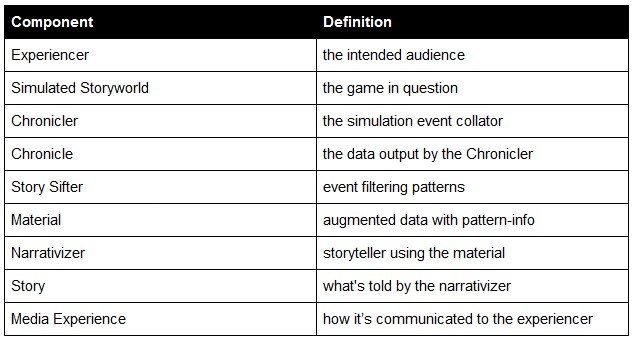
\includegraphics[width=\textwidth]{figures/4-Delve/curationist-architecture-components.jpg}
    \caption{A table of J Ryan's curationist architecture components.}
    \label{fig:curationist-architecture-components}
\end{figure}

%%%%%%%%%%%% END FIGURE %%%%%%%%%%%%%%%%%%%%%%%%%%%%%%%%

Some of these are somewhat extraneous to our purposes, but the critical components are the \textit{simulated storyworld} (the game itself), the \textit{chronicler} (the system collating and abridging game events), which outputs the \textit{chronicle} (a data object another system can operate on). What's left is a set of procedures to take on the role of \textit{story sifter} and \textit{narrativizer} to make use of the material to generate a story. Those roles are fulfilled by a prototype created in 2014 called \textit{LegendsWriter}, which operates as a component within LegendsViewer. We will return to this in more detail in Section \ref{subsubsec:legendswriter}.

\subsection{Expressionist}
\label{subsec:expressionist}

Now that we've shown some related work in simulation-driven narrativization---which covers how we acquire the \textit{chronicle}, or data object with simulation events---we can talk about how we translate that for \textit{Delve} in order to be narrativized.

This was accomplished using Expressionist, a grammar system created by J Ryan \cite{ryan2016expressionist}. Expressionist is used in several of Ryan's works, including Talk of the Town \cite{ryan2016characters} and Sheldon County \cite[p.~647-681]{ryan2018curating}. For \textit{Delve}, it was used as part of the event generation pipeline, specifically the surface text generation for character memories, and controlling how they change given player interactions.

Expressionist is an authoring system for context-free grammars \cite{bundy1984catalogue} that allow tagging on their nonterminal symbols. The tagging capability of the system puts it conceptually close to Knuth's attribute grammars \cite{knuth1968semantics}, but with the key difference that Expressionist grammars attach tags to its nonterminal symbols, not the production rules themselves.

Expressionist operates as part of a duo that together make a dynamic text generation system. Expressionist is Ryan's term for the editor that facilitates authoring, and the data structure exported from it. Productionist is a general term for the system that generates text from an Expressionist-authored grammar, and is thus called from the game’s code. Some implementations of Productionist pre-render text for different combinations of tags, so that at runtime generation becomes a lookup rather than search. While the authoring tool of Expressionist (and the data object it outputs) remain relatively the same no matter how the systems are using them, each Productionist is in practice a handcrafted, customized module that crosses that last bridge to output the necessary text, though Ryan provides an example implementation of Productionist in the public repo.

Text is generated using this system by sending a ``content request" to the Expressionist data object. This content request is composed of tags, or even hierarchies of tags, which can also be fine-tuned as ``required", ``desired" (with a simple scoring metric applied), or ``prohibited." The returned data is then processed by the custom Productionist module.

Because Productionists are custom to each implementation, they can vary widely. For example, tags on nonterminals don't necessarily have to be simple semantic strings like ``angry", ``sad", etc. They can even be code, as with Jonathan Lessard and the \textit{LabLabLab} collective's game Hammurabi \cite{lessard2017striving}. In their implementation, the ``code tags" decorating the nonterminals returned in response to queries were executed to affect the state of the game.

While not as complex as that use case, \textit{Delve} makes use of simple semantic tagging, which is later processed and translated through an ontology to new values, and then subsequently operationalized (discussed later in Section \ref{subsubsec:delve-writing-the-generative-grammars}).

This system is powerful, flexible, and expressive. But what about the combinatorics? Surely the ballooning number of combinations makes doing live queries a nightmare! This problem is solved by a third module, bundled in with Expressionist when it does its data export, called Reductionist. This module reduces the massive combinatorial space of potential grammar outputs to an optimized format that allows queries to be made quickly across the total tag combinations. It accomplishes this by ``semantically compressing" combinations to just ones with unique sets of semantic tags, bundling all the ``recipes" possible within that.

When a content request is made to the data object, the search can happen quickly to get to these groupings of recipes. And because the only text output processing is through the semantic tags, operationally it can treat any recipe it uses from that family as a valid answer to its query. The granularity of the tagging is left to the author, so if they find that certain things are returned as valid satisfactions to a tag set query that seem amiss or out of place (such as an angry reply when what was needed was an angry question) then what is required is higher definition on the tagset and tagging of the Expressionist nonterminals.

Because of Reductionist, it remains feasible to do run-time Expressionist queries for text generation despite its combinatorics, which is critical when it's used for dynamic dialogue or other instances where player interaction has changed the state space, and thus the types of tags required in queries.

\subsection{Computational Metaphor}\label{subsec:computational-metaphor}

Between simulation events and Expressionist tags, \textit{Delve} has a rich expressive state to use. But also at play with those tags is their embedding within an ontology, which is subsequently leveraged for metaphoric connections between concepts, and used to instantiate memories as physical objects, which the player can manipulate. For example, a sad memory may be tagged with the concept ``sad", which may route through the ontology to ``blue", which then grounds out in a ``blue rose" asset, which the player can interact with.

\subsubsection{Ontologies}\label{subsubsec:delve-ontologies}

When speaking of \textit{Delve}'s ontology, it's meant in its computer science context. Specifically:

\begin{quote}
    a set of representational primitives with which to model a domain of knowledge or discourse. The representational primitives are typically classes (or sets), attributes (or properties), and relationships (or relations among class members). The definitions of the representational primitives include information about their meaning and constraints on their logically consistent application. \cite{liu2009encyclopedia}
\end{quote}

%%ontologyDef%%
The core connection between \textit{Delve}'s two families of content--text memories and 3D objects--is mediated by the ontology. The core interaction of the game--manipulating the objects to change memories--relies on the players gradually understanding those connections through experimentation and play, then leveraging that knowledge to affect specific transformations. Because this desired gameplay relies on--and is driven by--the ontology, we say \textit{Delve} is an \textit{ontology-driven game}.
%%ontologyDef%%

Other games in this ontology-driven space occupy a unique intersection between the field of knowledge representation and computational media, in most cases utilizing their ontologies to procedurally generate content. While there are only a few examples, some games have successfully integrated this area of knowledge engineering into the core mechanics of their game.

\paragraph{\textit{Scribblenauts Unlimited}}\label{par:scribblenauts-unlimited}

%%%%%%%% BEGIN FIGURE %%%%%%%%%%%%%%%%%%%%%%%%%%%%%%%%%

\begin{figure}
    \centering
    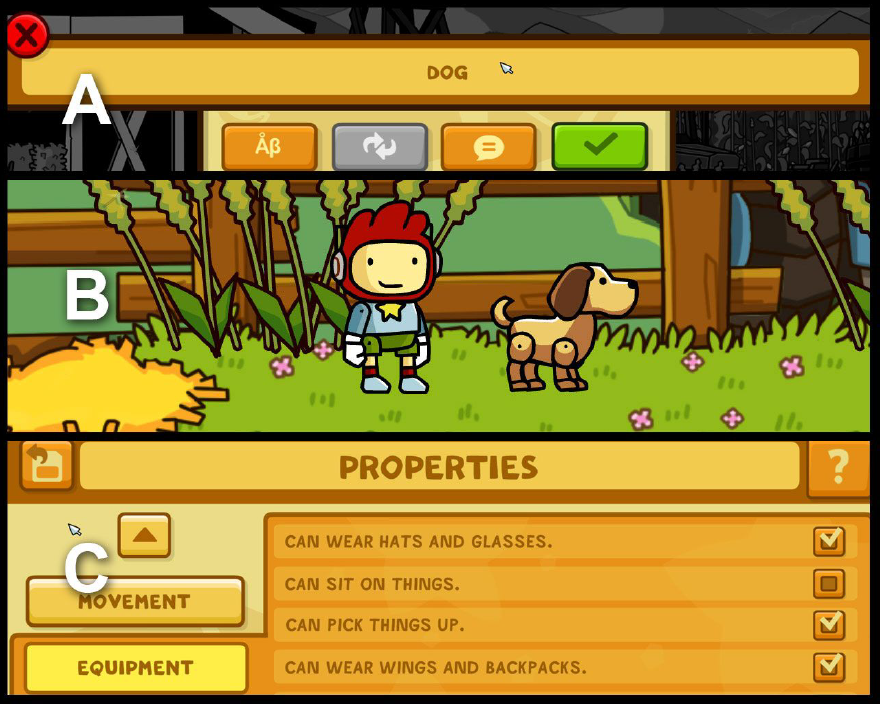
\includegraphics[width=\textwidth]{figures/4-Delve/scribblenauts.png}
    \caption{Three screen areas of \textit{Scribblenauts Unlimited}, where players type a word into their magic notepad (A) and it is instantiated in the world (B). They can also edit its properties using the Object Editor (C).}
    \label{fig:scribblenauts}
\end{figure}

%%%%%%%%%%%% END FIGURE %%%%%%%%%%%%%%%%%%%%%%%%%%%%%%%%

\textit{Scribblenauts Unlimited} is an ontology-driven game in which you solve puzzles through virtue of the main character's magic notepad. As shown in Figure  \ref{fig:scribblenauts}, the player can type in almost any word imaginable (A), and instantiate it in the game (B). The central thrust of the game is that players find emergent solutions to puzzles through the use of different objects, singly or in combination.

These objects are described in the Objectnaut database according to a schematic including ``around 40 key properties to determine an object’s behavior, including physical properties, material, electricity, temperatures, and many more attributes" \cite{tringali_2009} and are editable in the game (C in Figure \ref{fig:scribblenauts}). This database was adapted in size to be as large as possible and still fit on the target platform (Nintendo DS, iPhone, PC). At full size it has more than 10,000 unique entries.

Content is instantiated via a procedural animation system and 2D sprites. Limbs, wings, heads, and other parts each exist separately and can be modified and recombined, as can the color of each item. 

In terms of the gameplay, it's focused entirely on puzzle solving, which can only be accomplished through summoning objects or modifying objects in-game using the notepad. As a matter of fact, there are few verbs afforded to the player outside writing in the notepad, relating mostly to movement or attacking. Thus, the ability to solve puzzles is driven by an understanding of the properties of objects.

\paragraph{\textit{Argument Champion} and \textit{Dreamer of Electric Sheep}}\label{par:argument-champion}

\textit{Argument Champion} makes use of ConceptNet nodes and edges to determine valid logical connections between a starting concept and a goal concept, with the in-game purpose of convincing an audience that either your character's position on said concept is defensible and good, or that your AI opponent's position on a concept is bad \cite{smith_2012}. Harnessing ConceptNet, while notoriously problematic, lends the game an ontological model of over 1.6 million concepts and relations \cite{liu2004conceptnet}. As seen in Figure \ref{fig:dreamer-of-electric-sheep}, the words themselves are grounded out as direct printouts to the screen, contextualized as part of a speech. And the player's understanding of ConceptNet's somewhat quixotic conceptual relations directly translates to more successful arguments and a higher score.

%%%%%%%% BEGIN FIGURE %%%%%%%%%%%%%%%%%%%%%%%%%%%%%%%%%

\begin{figure}
    \centering
    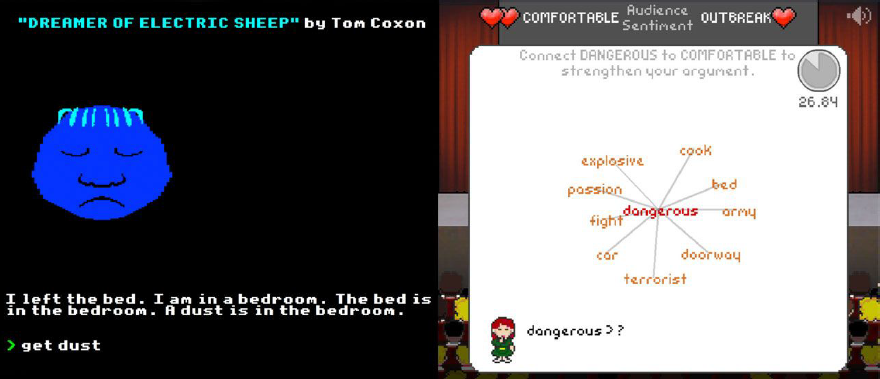
\includegraphics[width=\textwidth]{figures/4-Delve/androids-sheep.png}
    \caption{Sample output from \textit{Dreamer of Electric Sheep} (left) and \textit{Argument Champion} (right).}
    \label{fig:dreamer-of-electric-sheep}
\end{figure}

%%%%%%%%%%%% END FIGURE %%%%%%%%%%%%%%%%%%%%%%%%%%%%%%%%

\textit{Dreamer of Electric Sheep} follows a similar pattern, importing a subset of ConceptNet and then using certain connecting relations between nodes to afford actions reminiscent of interactive fiction parsers to the player (look, enter, leave, take, drop, give). Like \textit{Argument Champion}, it grounds out the representations as words on the screen that are put into sentence descriptions (Figure \ref{fig:dreamer-of-electric-sheep}). The player’s understanding of the network helps inform their actions in the game.

\paragraph{\textit{Imaginarium}}\label{par:imaginarium}

\textit{Argument Champion} and \textit{Dreamer of Electric Sheep} both make use of a very large third-party ontology (ConceptNet) and \textit{Scribblenauts} makes use of an ontology that, while hand-authored, still has over 10,000 nodes. \textit{Delve}'s ontology authoring approach, however, has more in common with approaches such as Horswill's \textit{Imaginarium} system \cite{horswill_2019}. \textit{Imaginarium} is intended as a tool for creating smaller, ad hoc ontologies for tabletop RPGs. While many ontology authoring interfaces can be complex and daunting for those unfamiliar with the space, \textit{Imaginarium}'s goal is to make that task easy enough to approach that of a casual creator \cite{compton-iccc2015}. Similarly to that, the ontology authoring in \textit{Delve} is intended to be as frictionless as possible (elaborated on in Section \ref{par:delve-implementation-the-substrate}), and authored as a way to additively connect nodes (be those Expressionist semantic tag nodes or nodes corresponding to objects and physical properties) together to facilitate the translation from memory surface text to memory palace object. However, in contrast to \textit{Imaginarium}'s interface which is evocative of natural language input, \textit{Delve} requires the user to input JSON data structures. Additionally, \textit{Imaginarium} is constraint-based, which means the data and output are guaranteed to be well-formed, whereas no such guarantees can be said about \textit{Delve}'s ontology (although that may become necessary in the future, once authoring has begun in earnest).

\subsubsection{Metaphor Systems}\label{subsubsec:metaphor-systems}

One way to drive the player to more directly engage with an ontology-driven experience is to complexify the conceptual relations, in turn requiring deeper interpretive work on the part of the player to understand. This increased engagement would (hopefully) map to increased proficiency in game tasks. In \textit{Scribblenauts} and \textit{Argument Champion} this is not the case: the instantiation of the content is a 1-to-1 correlation, the ontological frameworks largely representational, their relations descriptive of real-world qualities the objects possess. If you type ``dog" in the notepad in \textit{Scribblenauts}, it will make a cartoon version of a dog.

However, games need not be limited to literal ontologies to drive their procedural systems. There is a rich field of experiences to be created by grounding out more complex ontological relations to game assets and behaviors, and thus encourage player engagement with the underlying system.

The field of computational metaphor has insights to provide in this vein, particularly the early work of Fox Harrell and Jichen Zhu. Harrell's \textit{Alloy} and later \textit{Griot} system, and Zhu's \textit{Riu} system have been successfully used to create computational media works, grounding out their roots in semiotics and semantic theory into playable experiences.

\paragraph{\textit{Alloy} and \textit{Griot}}\label{par:alloy-and-griot}

Conceptual blending provides a methodology for combining and making connections between these frames or mental spaces, a process occurring all the time in our ``backstage cognition" \cite{fauconnier2001conceptual}.

Harrell’s \textit{Alloy} system took this conceptual blending model and translated key aspects of it into a computational model, implementing it through Goguen’s algebraic semiotics approach to blending \cite{goguen2010style}. It takes as input the data structures of the conceptual spaces and the maps between them, and outputs a diagram of a blended space, complete with mappings. A key insight here is that Harrell was not positing a sort of ground truth for these mappings as one might with symbolic AI approaches, but instead performing operations on subjective conceptual networks, which must be explicitly given to the system, pre-baked with the programmer’s preconceptions \cite{harrell_2007}.

Harrell iterated on \textit{Alloy} to create the \textit{Griot} system, which was used initially to generate his
``polymorphic poetry" works, such as \textit{The Girl With Skin of Haints and Seraphs} \cite{harrell2005shades}. This again was drawing from Goguen’s theories of algebraic semiotics to describe the sign systems involved. \textit{Griot} operated on ``theme domains", which were represented as ontologies of axiom sets relating to a specific theme. The \textit{Alloy} algorithm would then operate on those theme domains to translate between them, and then ground out the result through ``media morphisms" (which in these initial works was natural language, but in later instantiations incorporated graphics).

Additionally, Harrell also added a new type of automaton called a ``probabilistic bounded stack transition machine", or ``event structure machine" to select how the phrase templates for output were composed and arranged \cite{goguen2010style}. This sort of translation and systemization of theory-based models is very powerful, providing a way to ``ground out" the implications of the theory, to test its limits and confront its implications.

\paragraph{\textit{Riu} and Force-Dynamics}\label{par:riu-and-force-dynamics}

Zhu’s \textit{Memory, Reverie Machine} also used axioms selected from different ontologies for blending through \textit{Griot}, and applied the result to ``experiences of events, objects, and actors to affective concepts determined by current state, in this case emotional state, of the protagonist" \cite{zhu_harrell_2011}. This grounded out in the textual display of memories, which were annotated based on their subject, and retrieved through actions of the main character, the robot Ales. Zhu’s later work \textit{Remembrance} applied this approach to perform changes to the environment around the protagonist based on their current emotional state, which could result in changes from a well-lit room with cheerful music and nice furnishings to a darker room with dirtier, more bedraggled objects and more ominous music \cite{zhu2011representing}.

Another thread of work pursued by Zhu is the \textit{Riu} system, whose approach to computational analogy, specifically story representation, draws from Talmy’s theory of force-dynamics, as opposed to \textit{Griot}’s conceptual blending roots. Force-dynamics allows the formulation of graded relationships between entities, which allows more expressivity when modeling them for the purposes of story planning \cite{zhu2010story}. The particular component of this system most pertinent to \textit{Delve}'s development is \textit{Riu}’s Structure Mapping Engine (SME). 

The SME is what computes the similarity level between two ontological domains in this work, on both a surface and structural level, informed by Gentner’s structure mapping theory. \textit{Riu} uses a two-step process, starting with a surface level comparison of keywords in each content segment, and pulling out some number which have the highest level of tag overlap. Secondly, it uses structure mapping to determine on a deeper level which one of the selections provides the most similar translation into the new domain. Taking a cue from other systems, \textit{Riu} does this so that the second, computationally expensive operation is only called on a list of comparisons filtered by the shallower, yet faster, selection process.

Zhu’s later work with Ontañón pushed the idea of this mapping further through the SAM (Story Analogies through Mapping) algorithm \cite{ontanon2011sam}. SAM provides a vector for including domain knowledge in the process of generating analogous stories to the input, allowing a story with certain ontological content to be metaphorically translated across different domains.

\subsection{Summary}\label{devel-related-summary}

In summary, we've seen threads of work addressing simulationist narrativization---the practice of third-party narrative generation using data from separate systems as input, then creating narratives to enhance said systems' experiences. These works range from automated sportscasters and embedded agents in FPS games (which narrate while events happen live) to automated sports journalism systems and the use of story intention graphs to formally represent game playthroughs (narrated after play has concluded).

We then looked at Expressionist \cite{ryan2016expressionist}, J Ryan's system for semantically tagging grammars used for dynamic surface text, which is used in \textit{Delve} for character memories.

We then looked at ontology-driven games, to get a sense of related systems that have incorporated this knowledge engineering approach into their game systems. Like those, \textit{Delve} uses a simple ontology that bridges Expressionist tags with 3D game objects (which we'll explore in Section \ref{par:delve-implementation-the-substrate}). This process of computational metaphor puts it in dialogue with previous works like Harrell and Zhu's, though for our purposes our ontology is a less rigourous, and more hand-authored one.

The concept of ontology-driven gameplay through computational metaphor is one which has been with \textit{Delve} since its first conception. However, the method for how character memories are generated has gone through iteration. This iteration was mostly carried out in a previous project \textit{LegendsWriter}, while some other potential applications were explored in \textit{Argosy}. We will next briefly look at these projects, to help clarify how the event generation strategy in \textit{Delve} was solidified.

\subsection{Prior Works}\label{subsec:delve-prior-works}

\subsubsection{\textit{LegendsWriter}}\label{subsubsec:legendswriter}

As with the earlier-mentioned simulationist narrativization works, the basic premise of \textit{LegendsWriter} is that game data from a high-fidelity simulation provides a body of causally-linked, domain-constrained events as the raw material for story generation (here conceived of as narrativization). Because the generated events follow a rigorous simulation logic, the ``facts" of the stories are already baked in. We can rely on the simulation to only give us causally consistent events, not ones where, for example, the main character dies in the middle, or somehow is in two places at once, etc. The conventions of the simulation logic are the bare minimum conventions of the storytelling about that world, so they do the heavy lifting.

Note that in plan-based story generation, much of the effort of domain modeling is precisely in authoring operator preconditions and effects to correctly model the causal structure of the domain. But using the narrativization paradigm, our attention can turn to focusing on the aesthetics of narrative structures and tropes. Even though the other systems presented in this dissertation, \textit{Ice-Bound} and StoryAssembler, are not classic story planners, they too depend on the correct chaining of preconditions and effects (as well as clever state-based templating) to achieve causal coherence. \textit{LegendsWriter} gets this causal coherence for free, through virtue of the simulation it uses as input. 

The high-fidelity simulation we targeted for this was \textit{Dwarf Fortress}, and the third-party program LegendsViewer. LegendsViewer already provides simple descriptions for exported \textit{Dwarf Fortress} character events in LegendsViewer are one-line sentences, such as ``In 96, Almo confronted the night creature Ayanu Cryptmurk in the Tomb of Dusk." A selection of such a chronicle can be seen in Figure \ref{fig:legendsviewer}. When the events are read in sequence, they definitely suggest a story unique to the character involved, approaching something akin to Tale-Spin, the descriptions of sport games, or a medieval chronicle. The bones exist, but there's no meat, no leveraging of dramatic build-up. That is left as an exercise to the reader.

%%%%%%%% BEGIN FIGURE %%%%%%%%%%%%%%%%%%%%%%%%%%%%%%%%%

\begin{figure}
    \centering
    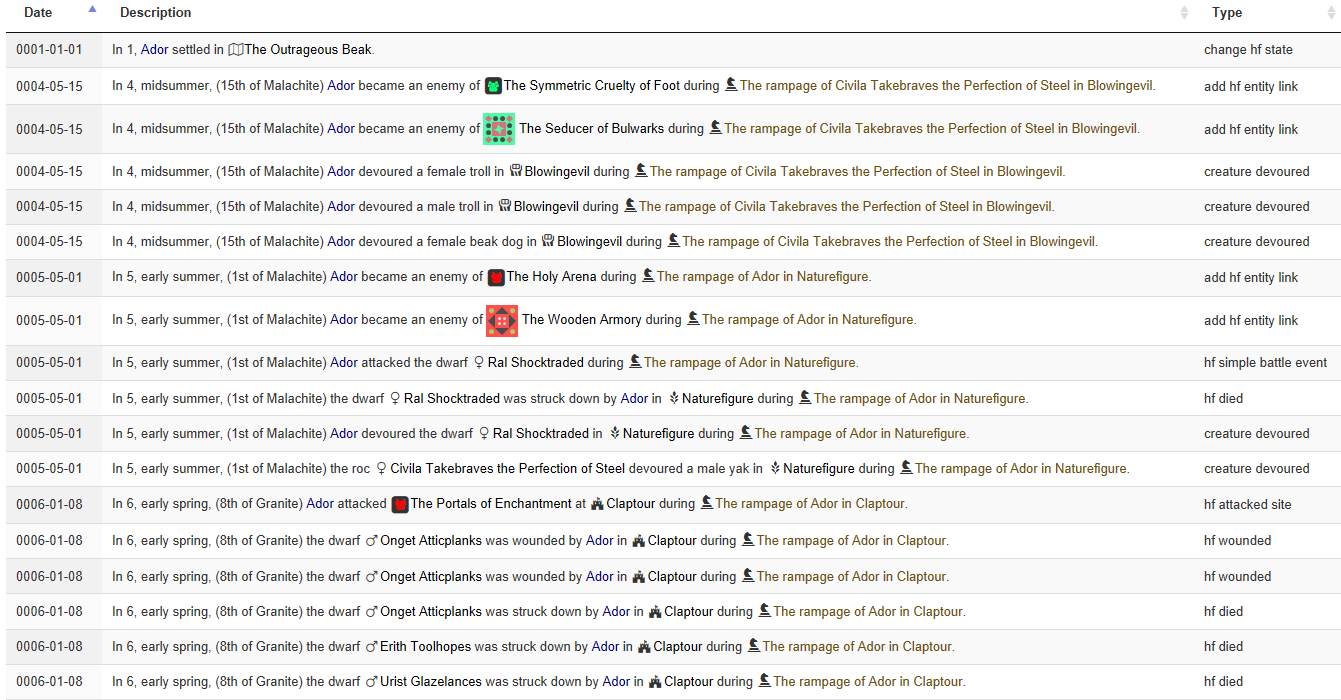
\includegraphics[width=\textwidth]{figures/4-Delve/legendsviewer.png}
    \caption{A view of character life events in LegendsViewer.}
    \label{fig:legendsviewer}
\end{figure}

%%%%%%%%%%%% END FIGURE %%%%%%%%%%%%%%%%%%%%%%%%%%%%%%%%

Thus, if we adopt the curationist architecture for this (Figure \ref{fig:curationist-legendsviewer}), we can use \textit{Dwarf Fortress} as our \textit{simulated storyworld}, the exported legends data as the \textit{chronicle} (facilitated by the third-party program DFHack) and create a new system (\textit{LegendsWriter}) to process that to create stories. The \textit{story sifting} it uses to determine which stories to tell for which characters, is something we will return to in much greater depth in Section \ref{par:sifting-patterns}, where we discuss the approach in detail for \textit{Delve} event generation. For now, we can say simply that it looks for certain sequences of events (\textit{sifting patterns}) and if matched, it runs state-driven templates to create surface text of a \textit{story} from those event sequences.

%%%%%%%% BEGIN FIGURE %%%%%%%%%%%%%%%%%%%%%%%%%%%%%%%%%

\begin{figure}
    \centering
    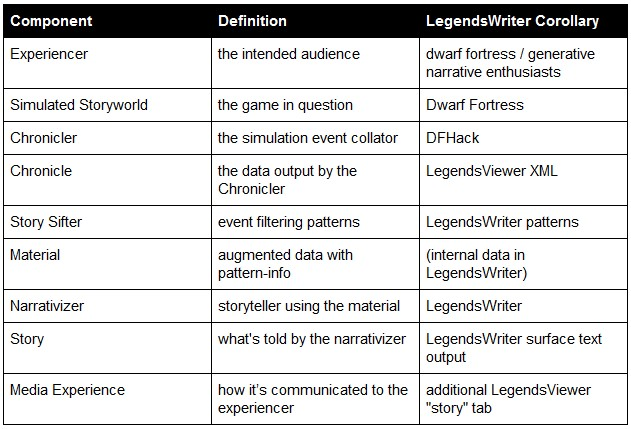
\includegraphics[width=\textwidth]{figures/4-Delve/curationist-legendswriter.jpg}
    \caption{A table of J Ryan's curationist architecture components, with their \textit{LegendsWriter} corollaries.}
    \label{fig:curationist-legendsviewer}
\end{figure}

%%%%%%%%%%%% END FIGURE %%%%%%%%%%%%%%%%%%%%%%%%%%%%%%%%

Though \textit{Dwarf Fortress} allows us to circumvent the ``causal coherence" problem, it presents a potentially even greater challenge of its own in the high resolution of its simulation. Character life stories can have anywhere from a handful to thousands of life events. Each one of these life events can be in one of 62 different categories (see Figure \ref{fig:DF-event-types}). Furthermore, each category may contain sub-categories, such as with ``hf change state." Depending on the state change, that category can encapsulate a character settling down in a new town, scouting locally for trouble, becoming a thief, hunting for food, becoming a kidnapper, or any combination thereof.

%%%%%%%% BEGIN FIGURE %%%%%%%%%%%%%%%%%%%%%%%%%%%%%%%%%

\begin{figure}
    \centering
    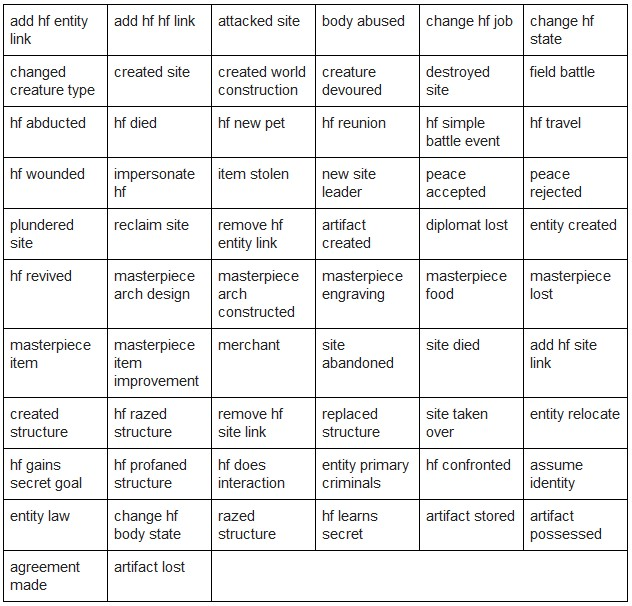
\includegraphics[width=\textwidth]{figures/4-Delve/dwarf-fortress-event-types.jpg}
    \caption{Different life event categorizations. ``HF" here means ``historical figure", a civilization or individual who has accumulated enough life events to merit recording in the Legends XML chronicle.}
    \label{fig:DF-event-types}
\end{figure}

%%%%%%%%%%%% END FIGURE %%%%%%%%%%%%%%%%%%%%%%%%%%%%%%%%

However, we don't need to solve all of \textit{Dwarf Fortress} to create interesting stories. We can start by covering subsets of event types as selected by a user.  Because LegendsViewer is available as an open source project, it was possible to modify its code directly, such that character events we pull out to narrativize are given a ``storyedness" amount. This amount can be determined by the author while writing---for example if they want to take significant time to build out a particularly elaborate story, they can give character events involved in it a ``storyedness" rating of 5. Smaller stories can be 1, and so on. These events can them be summed up per-actor, to give each actor a total ``storyedness" amount.

We can then add ``storyedness" as a filter to LegendsViewer's UI, which is already capable of navigating between characters. By adding an additional ``storyedness sort field" to the LegendsViewer interface, we gain the ability to pluck out only characters that possess rendered stories that we've authored content for. This approach means content can be authored incrementally, and we can see the exemplar stories by leveraging the existing LegendsViewer interface. Essentially, we gain event generation from \textit{Dwarf Fortress} ``for free", and leverage an existing well-developed project that allows us to sensibly navigate and filter the dataset. All that's needed now is to author the patterns.

\paragraph{\textit{LegendsWriter} Pattern Authoring}\label{par:legendswriter-pattern-authoring}

As can be seen in Figure \ref{fig:legendswriter-output}, these experiments with handcrafting story sifters centered around night creatures (vampires), a specific subset of \textit{Dwarf Fortress} characters. These were chosen as an initial focus for two reasons. One, such characters reliably have at least one sequence of events with three specific categories: ``hf gains secret goal: immortality", ``hf profaned structure", ``hf does interaction: deity curse." In \textit{Dwarf Fortress}, one becomes a vampire after desecrating a sacred site, and being cursed by a deity. This naturally lets us create a sifting pattern ``storyOfImmortality", composed of those three event categories. The second reason is that night creatures are immortal. Unless meeting a grisly end, their lives typically contain several hundred events. This gives us a wider variety of events to filter, thus increasing the chances that our patterns match. This makes the bar for catching things in our sifting patterns very low, which is good for exploratory prototyping.

% \begin{quote}
%     In the year \textbf{121}, \textbf{as summer withered into fall}, trouble found \textbf{\underline{Rakust}}. It was in \textbf{\underline{Painttarget}}, where members of \textbf{\underline{The Humid Lance}} accused \textbf{\underline{Rakust}} of \textbf{murdering a local}. \textbf{Ironically,} \textbf{\underline{Rakust}} \textbf{had not murdered anyone...in \textbf{\underline{Painttarget}}, at least. Her} accuser stepped forward and \textbf{laughed unpleasantly. ``To kill is a terrible crime."} \\
% \textbf{\underline{Rakust} flicked her eyes} to the \textbf{grumbling} crowd. \textbf{``What is that supposed to mean to me?"} \\
% \textbf{After muttered imprecations}, the \textbf{locals dissipated}. \\
% After that, \textbf{\underline{Rakust}} decided discretion was needed, and so left \textbf{\underline{Painttarget}} to settle in \textbf{\underline{Championgirders}}. \\
% For \textbf{a while things were quiet, but once again \underline{Rakust}'s past, or at least reputation, would come back to haunt them}. This was \textbf{four} years later, \textbf{in spring, when the crocuses had just sprouted}. Everything had been uneventful since she'd re-settled in \textbf{\underline{Championgirders}}. \\
% Then one day, there was a knock at the door. \textbf{\underline{Rakust}} opened it, to reveal \textbf{most of \underline{The Fortification of Truth}}, who immediately accused her of \textbf{murdering some nobody}. Ironically, \textbf{\underline{Rakust} had not murdered anyone...in \underline{Championgirders}, at least. Her} accuser stepped forward and \textbf{glowered. ``We don't take kindly to murderers here."} \\
% \textbf{\underline{Rakust} swallowed carefully. ``I'm sure I don't know what you're talking about."} \\
% After \textbf{a few minutes of hot silence, the mob dispersed}.
% After that, \textbf{Rakust} decided discretion was needed, and so left \textbf{Championgirders} to settle in \textbf{Foggyrims}.
% \end{quote}
%%%%%%%% BEGIN FIGURE %%%%%%%%%%%%%%%%%%%%%%%%%%%%%%%%%

\begin{figure}
    \centering
    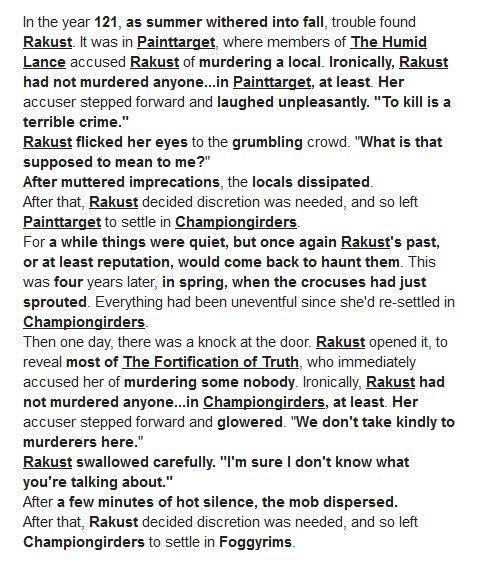
\includegraphics[width=\textwidth]{figures/4-Delve/legendswriter-output.jpg}
    \caption{Example \textit{LegendsWriter} output. Bold words are dynamic. Underlined words are simulation entity references.}
    \label{fig:legendswriter-output}
\end{figure}

%%%%%%%%%%%% END FIGURE %%%%%%%%%%%%%%%%%%%%%%%%%%%%%%%%

\paragraph{Procedural Subjectivity}\label{par:procedural-subjectivity}

This approach could also facilitate the creation of a system where there is a subjective notion of history, and those notions can be unique to different character perspectives, as we saw adapted with the sports commentators in Rocco and Byrne \cite{andre2000three}. Originally, \textit{LegendsWriter} was titled ``Dwarf Grandpa", because the idea was that simple filtering metadata could be added to the sifting patterns, such that a ``farmer grandpa" or ``battle-worn grandpa" etc would have different sifting pattern pre-conditions, and thus yield different stories from the same set of events.

The combination of hierarchical nesting along with ``role-based narrator" preconditions on sifting patterns could be an incredibly powerful design pattern to use in dynamic narratives. While it remains the domain of future work, one can easily imagine a set of global patterns that can be applied, then culture-specific patterns nested beneath that, then character-specific patterns, then state-specific patterns. For example, a character could relate a story who reads lots of romances. If one wrote many patterns with ``romance" tags, then when you have a player ask them to describe a brooding, aloof character, they may come up with a very different interpretation of said character’s history than if you asked someone who hates people that brood. None of the actual motivations or things referenced in the event text need necessarily be modeled in the simulation, so long as they’re consistent to the narrator.

This technique could be potentially used to create conflicting accounts that, critically, conflict in consistent ways. You could have two characters witness a murder, one who’s a pessimist, and another who believes in justice in the hereafter. When asked to describe the event, the pessimist would consult their library of patterns, output the text ``Someone was murdered–which just goes to show that life is short and brutal." and you could surface why to the player with something like ``(Char1 is a pessimist)." The other character would have access to patterns that would render text ``Someone was murdered–but the murderer will get what’s coming to them, in life or the hereafter" with the explanation ``(Char2 believes in justice in the hereafter)." Again, the power of this approach depends wholly on the sifting pattern library and narrativizer, which can be gated on groupings of characters on culture, socio-economic status, disposition, or even dynamic tags that happen as a result of the simulation, like ``survived trauma" or ``wonderful childhood." 

While only a preliminary amount of authoring was done with \textit{LegendsWriter}, it did provide fertile initial ground for exploring the technique of story sifting, and generating stories from particular sequences of simulated events. The techniques explored for this could be broadly categorized as ``top-down" and ``bottom-up", which will be covered in Section \ref{par:sifting-patterns}.

However, these patterns were matched automatically by the system, and getting to acceptable levels of ``event coverage", where many of the simulated events were able to be encapsulated by these patterns, proved very difficult. Getting to the point where readers could get an appreciable amount of interesting and diverse stories from \textit{Dwarf Fortress} events would take a lot of authoring. This prompted a different design approach for a later prototype, \textit{Argosy}.

\subsubsection{\textit{Argosy} and Sculptural Sifting}\label{subsubsec:argosy-and-sculptural-sifting}

In \textit{LegendsWriter} the application of sifting patterns was automatic, controlled by the heuristics and pre-conditions added to them when they were authored. As such, it isn't interactive, though it is generative.

In order to explore how sifting patterns can be shifted from a post-generation process to a core part of a game's mechanics, controlled by the player, a prototype game called \textit{Argosy} was created. 

The narrative framing is that you're an occultist who has been unexpectedly put in charge of a secret government lab of scientists, after your predecessor went mad. The scientists are working on a weapon to close eldritch portals, which have unexpectedly started opening all over the world. 

%%%%%%%% BEGIN FIGURE %%%%%%%%%%%%%%%%%%%%%%%%%%%%%%%%%

\begin{figure}
    \centering
    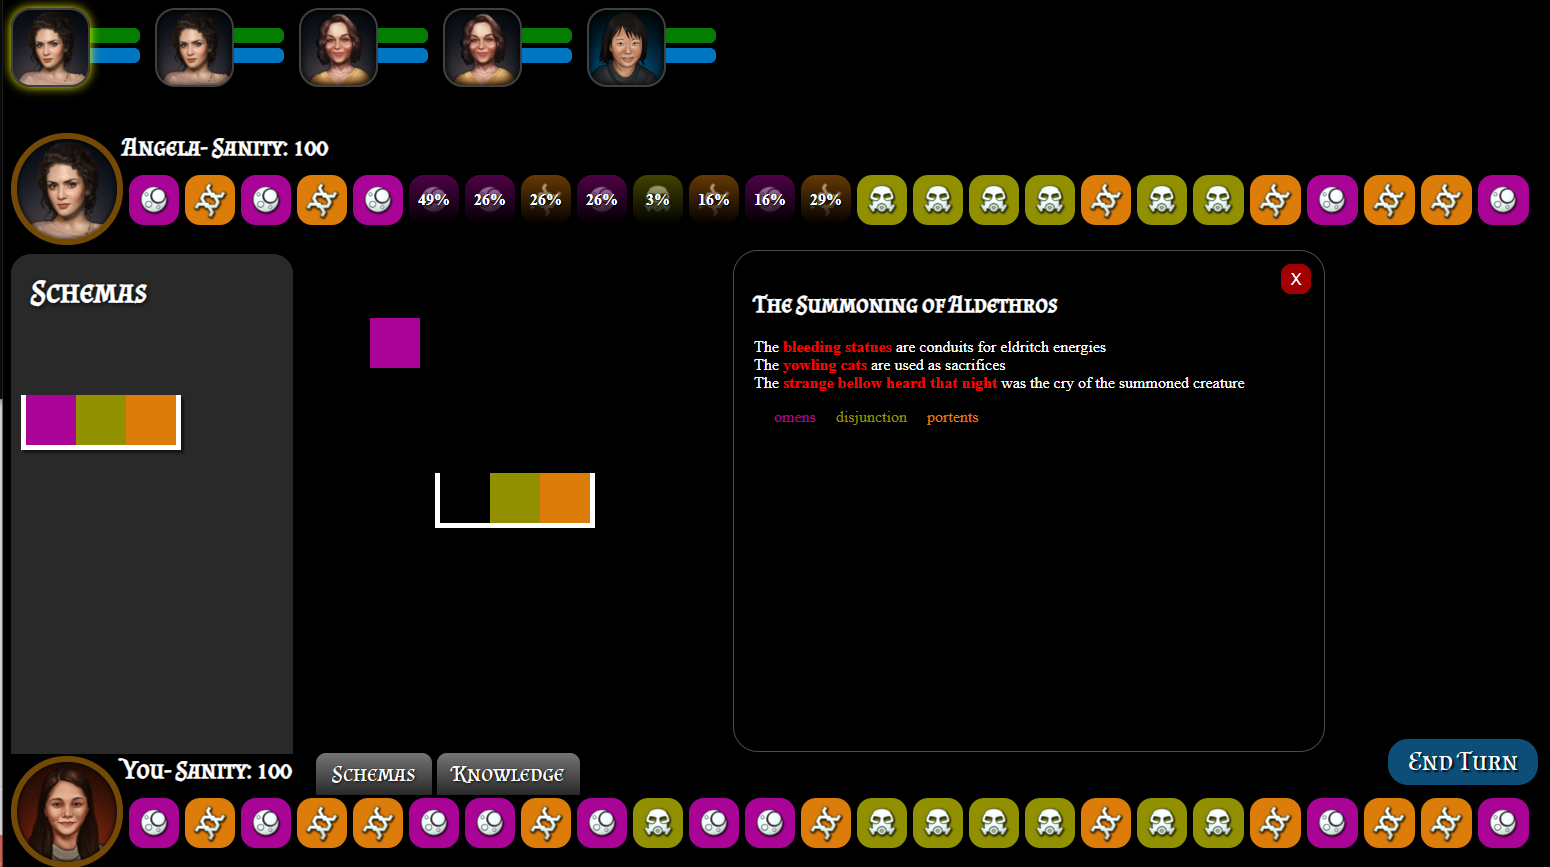
\includegraphics[width=\textwidth]{figures/4-Delve/argosy.png}
    \caption{Screenshot of \textit{Argosy}.}
    \label{fig:argosy}
\end{figure}

%%%%%%%%%%%% END FIGURE %%%%%%%%%%%%%%%%%%%%%%%%%%%%%%%%

At the end of each turn, each member of your team takes sanity damage from the number of ``unexplained events" on their timeline. As the leader and an accomplished occultist, you have access to ``supernatural schemas" which you can use to ``explain" a certain number of events, by allocating the schema to them. Your goal is for your team to survive a certain number of turns without going mad, so they can close the portals.

Mechanics-wise, each team member has their own timeline of events. Each event is one of five different types. At the end of your turn, each scientist takes ``unexplained event" sanity damage. If their sanity falls to zero, then they are removed from the game. If they survive, five new events are added to their timeline

Each turn you are granted some number of schemas (the in-game term for sifting patterns) which each have three ``anchors." The anchors' colors correspond to the event types. The player drags these anchors onto events matching that color on any of their scientists' timelines. When they do, the anchor connects to that event. When the player matches all three anchors to the timeline, the span of events covered by the schema are then ``explained." A simple heuristic is used for calculating the ``amount of explanation" that it affords, a linear falloff based on distance from the anchors. This prevents players from using a schema to simply cover an entire character's timeline from beginning to end.

As with \textit{Ice-Bound}, this game shows promise because of its systemic framing that sidesteps some of the pernicious authoring problems for combinatoric narratives. By framing the explanation of events with the schemas as a goal, we shift the player's role from generative narrative critic to constructive collaborator. System shortcomings (such as a lack of schemas that can adequately cover timeline events) are cast instead as deliberate designs for challenge, rather than an authoring failure.

\paragraph{Surface Text}\label{par:argosy-surface-text}

Because the usual concerns of how to accomplish coverage of events through story sifting patterns is set aside as a game mechanic, our main focus for this prototype is the surface text for events, and the explanations generated by putting schema anchors on events. The ``narrativizer" for \textit{Argosy} works through a combination of simple context-free grammars (using Compton's \textit{Tracery} library \cite{compton2015tracery}) synced between the event and the schema anchor. For example, an event might have the description ``The statues in Times Square started speaking in blood." after running the grammars in Figure \ref{fig:argosy-event-data} (in the field ``description"). A schema with an initial tag of ``omens" (like the one in Figure \ref{fig:argosy-event-data}) could put the first anchor on this event. When doing so, the hook in the event is populated to the schema, such that the ``explanation" field's first entry reads ``The statues are conduits for eldritch energies." If the anchor is switched to a different ``omens" event, it will likewise update.

%%%%%%%% BEGIN FIGURE %%%%%%%%%%%%%%%%%%%%%%%%%%%%%%%%%

\begin{figure}
    \centering
    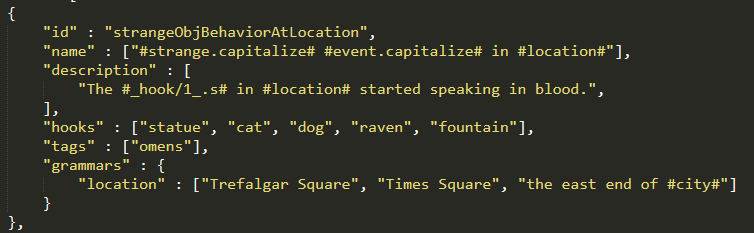
\includegraphics[width=\textwidth]{figures/4-Delve/argosy-event-data-object.png}
    \caption{\textit{Argosy} event data object, containing a ``hook" that is set in the ``description" that is used by anchors in schemas.}
    \label{fig:argosy-event-data}
\end{figure}

%%%%%%%%%%%% END FIGURE %%%%%%%%%%%%%%%%%%%%%%%%%%%%%%%%

%%%%%%%% BEGIN FIGURE %%%%%%%%%%%%%%%%%%%%%%%%%%%%%%%%%

\begin{figure}
    \centering
    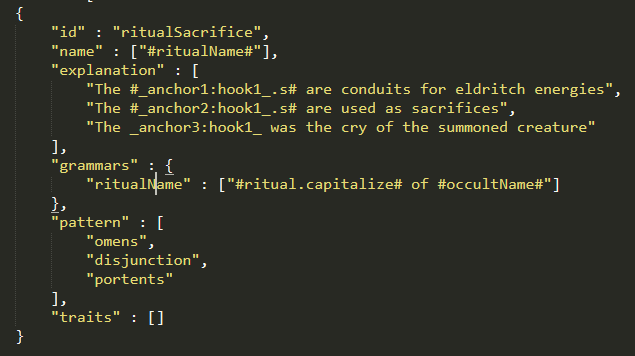
\includegraphics[width=\textwidth]{figures/4-Delve/argosy-schema.png}
    \caption{Data object for an \textit{Argosy} schema. The \_anchor1:hook1\_ syntax allows the explanation text to change depending on which event the anchor is attached to.}
    \label{fig:argosy-data-schema}
\end{figure}

%%%%%%%%%%%% END FIGURE %%%%%%%%%%%%%%%%%%%%%%%%%%%%%%%%

These schemas also have metadata, in the form of the ``traits" field, which are applied to scientists when a schema is applied to their timeline. These are simple flags which can be set as preconditions for further schemas. Therefore, using schemas on characters changes the characters, which can potentially impact which explanations are valid for them in the future, or perhaps even more game processes tied to different mechanics.

While only a prototype for now, this game design shows there are substantial ways that story sifting can be adapted to not only provide generative text for events that have already happened, but put the player ``in the loop" and expose part of the process as core game mechanics, and thus also avoiding some potential authoring pitfalls.

\subsubsection{Prior Works Summary}\label{subsubsec:delve-prior-works-summary}

These two experiences represent generative narrative internally, as well as externally through third-party programs. This allowed us to demonstrate two prototypes that leveraged ``curationist architecture" to tackle narrative generation in dialogue with the simulation systems. In the course of this we were able to explore authoring approaches for sifting patterns, which we'll return to in \textit{Delve} in the following section.

Bringing both Related and Prior Works together, we're now sufficiently positioned to talk about \textit{Delve}, an exploratory system that pre-generates history for its characters, in service of constructing a chronology of memories for each one. Those memories are instantiated in a 3D space (a ``memory palace") as user-manipulable objects. When the objects are changed, those changes then map back to the memories, changing the data representation, as well as the surface text.

\section{System Description}\label{sec:delve-system-description}

\textit{Delve}'s general architecture centers on the creation of a character "memory", which consists of a data object capable of generating text (marked up with references to accompanying 3D objects), given a set of requested semantic tags. Both the event generation system and the systems that enabled the manipulation of memories make this significantly more complicated than either\textit{ Ice-Bound} or StoryAssembler works by a wide margin. Furthermore, the authoring challenge these compounded combinatorics, constrained by the hierarchical event generation, pose is not one that's been fully grappled with yet. Because work is ongoing on the finer points of the system as well as non-prototype content, we'll talk about the current implementation details, as well as likely changes based on existing authoring experience with the system. In terms of Authorability, we'll discuss how applying analysis through the lens of its sub-categories informed where to spend authorial effort.

\subsubsection{Description of the System}\label{subsubsec:delve-description}

%%%%%%%% BEGIN FIGURE %%%%%%%%%%%%%%%%%%%%%%%%%%%%%%%%%

\begin{figure}
    \centering
    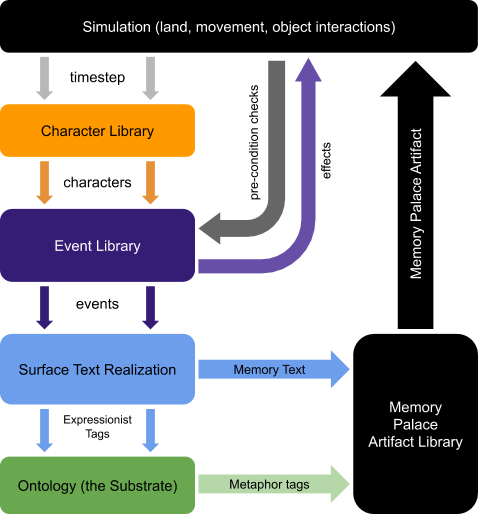
\includegraphics[width=\textwidth]{figures/4-Delve/delve-diagram.png}
    \caption{Flow between different systems in \textit{Delve}, moving from simulation timesteps to generation of a memory palace artifact from a character event.}
    \label{fig:delve-diagram}
\end{figure}

%%%%%%%%%%%% END FIGURE %%%%%%%%%%%%%%%%%%%%%%%%%%%%%%%%

%%GDoc comments%%
While refinement of core \textit{Delve} architectures is ongoing, the basic flow between its systems can be seen in Figure \ref{fig:delve-diagram}. The execution is as follows: when \textit{Delve} starts, it simulates events to fill some preset amount of ``timesteps." For each timestep, it goes through an ordered list of characters sorted by ``narrative power" (a simple metric set when they are generated) and pulls a valid event from the event library to cast them into. Event validity involves checking a precondition against the current simulation state. Once chosen, the effects for that event are run, modifying the simulation state. The event is then passed to the ``surface text realization" system. The Expressionist grammar is then run for that memory, and the memory text is stored. The semantic tags resulting from that output are sent to the ontology system (called the Substrate), which finds a valid connected concept node corresponding to a physical objects. Then, both the memory text and concept nodes are sent to the Memory Palace Artifact Library, which instantiates the 3D object in the scene, along with the object transformations that can be applied to it. These object transformations are paired with their corresponding text transformations, such that the system can modify the text of the memory to match the object state, if the player changes it.
%%GDoc comments%%
Once the simulation of all characters' histories is complete, the player can then ``delve" a character, which displays the rooms of their memory palace, with the memory objects instantiated. The player can then select objects and read the corresponding memory. They can also change the object in certain ways---such as transmuting the material or moving it---which in turn affects the memory text.

\subsection{Core Architectures}\label{subsec:delve-core-architectures}

\subsubsection{Land and Prop Generation}\label{subsubsec:land-and-prop-generation}

Before the player can navigate character memory palaces, the characters need memories. And in order for characters to have memories, they need some model of location where those memories take place. So we need to generate some areas.

Because the main focus of \textit{Delve} is on the complex mapping of possibility space to surface text generation for memories, the underlying simulation is of less initial importance (though for future work this is obviously a rich area to increase generativity of the system). As such, the land generation is kept as simple as possible. Land is divided up into ``areas", which have a type, such as ``forest", ``mountain", or ``plains." Each area is also populated by props, which are treated by the system as---and have similar properties to---characters. The key difference is mostly an authoring convention in that they lack volition (i.e., they can't initiate events, and are not required to have every timestep fulfilled). However, the system supports casting them into events, such that---for example---a specific prized possession can be stolen from one character by another. This architecture choice also means that once the history has been generated, objects can be potentially queried to see what their ``story" is.

Each area is connected to at least one other area, and then further connections are layered in. These connections are labeled as ``leylines", because---unlike traditional physically-based roads or paths---area connections are intended to be mutable and non-physical, relying more on the changing of their inhabitants or game state to determine which are connected and which not. This also avoids getting bogged down in topological map generation code, as that is a solved problem outside the main concern of the project.

The main capability this adds is the ability of characters to move to other locations, and initiate events with other characters that are in the same area as them. It also populates areas with concept nodes that tie to the ontology (e.g. forest, mountain, plains, etc) which can be leveraged if necessary as hooks for later additions to the generative systems.

\subsubsection{Character Generation}\label{subsubsec:delve-character-generation}

Initial character generation is still a somewhat nascent system in \textit{Delve}, but there are two pertinent characteristics which touch the other systems, and are designed to have an integrated impact on the initial history generation.

\paragraph{Domains and Dominions}\label{par:domains-and-dominions}

Characters start out with an initial domain in which they possess a small integer amount of influence. These domains are flagged entities in the ontology, which connects the event generation and memory object / palace system. Domains are concepts like ``fire" or ``iron" or ``laughter." If a character has the most points in a given domain, they are said to be the ``Dominion" of that concept. When any events happen with output text containing semantic tags relating to a domain, the associated Dominion accrues some amount of ``favor" from the characters participating in the event. 

While purely a design convention, in practice this is meant to facilitate stories where Dominions become more and more powerful, until they ``call in their favor" with another character, usually to their benefit. Other events can be triggered whose effects lower a particular character's domain score, thus producing a give-and-take dynamic.

Eventually, this system is meant to provide the backbone for the game's main player interaction. The manipulation of memories results in different semantic tags being active for said memories, which can then result in a given character losing or gaining their Dominion. Characters approach the player with ``quests" to find a particular character, delve their memories, and change them correctly to correspond to desired domains.

\paragraph{Relationships}\label{par:delve-relationships}

Characters also start with an initial relationship with another character, to facilitate events which might have a relationship casting requirement. Most of the planned events in \textit{Delve} require more than one character, and who is cast into the supporting character role will often be driven by relationships.

Relationships in \textit{Delve} have an associated concept node and a strength between 0 and 1. This means that a relationship isn't limited to the typical fare of friendship, love, or hatred. This is intended to capture more nuanced and specific relationships, such as someone who buys bread every day from a baker developing a “bread” relationship with the baker. Relationships can also be between characters or props. This allows a character to, for example, have a relationship with their sword with the concept ``murder." This is intended to provide more hooks for event casting to latch onto, and provide more interesting granularity between characters as the history generation plays out. For example, one might imagine a character who is the Dominion of ``revenge" setting the player a quest to change another character's relationship with their favorite sword such that the associated concept is ``revenge", so that the Dominion can demand it be given to them.

\subsubsection{Event Generation}\label{subsubsec:event-generation}

With this simple layout of lands accomplished, and some initially seeded characters, we can now talk about event simulation. We knew the strategy ultimately selected for event generation and narrativization would be one of the key underpinnings of \textit{Delve}, and greatly impact both the character of the system, and thus the authorial leverage of content authoring for it. Therefore, much time was given to exploring the ramification of different approaches. Specifically, these different approaches are for the application of \textit{sifting patterns}, which we will first define and cover in detail. We will then cover the two broad categories of approach: bottom-up (which was ultimately abandoned) and top-down (which was ultimately chosen). Once we've established that, we can then broadly talk about the generation procedures (beginning with Section \ref{par:delve-generation-procedure}).

\paragraph{Sifting Patterns}\label{par:sifting-patterns}

As mentioned in earlier sections, \textit{sifting patterns} is a term coined by J Ryan as part of his curationist architecture \cite[p.~249-250]{ryan2018curating}. It specifies a pattern---be that regular expression or otherwise---used to filter raw sequences of events, such as from a chronicle export of a simulation. The \textit{sifting pattern} draws out the events for a story, and the \textit{sifting heuristic} scores those sets, or guides the initial pattern. These heuristics can be simple or complex, depending on whether creators want to spend focus on the initial sifting as the point of refinement, or on subsequent processes (such as state-driven templating or grammars) to refine the output from rougher-grained sifting once that occurs.

Sifting patterns can be wholly automated, authored and executed with no input from the player, as we saw with \textit{LegendsWriter} in Section \ref{subsubsec:legendswriter}. They can also exist in dialogue with players, such as with the \textit{Argosy} prototype in Section \ref{subsubsec:argosy-and-sculptural-sifting}, or Kreminski et al's system \textit{Felt}, which ``assists players in the process of narrativizing their play experiences by helping them locate sites of potential narrative interest in a larger simulated storyworld" \cite{kreminski2019felt}.

In a way, sifting patterns can also be thought of as siblings of playtraces, which in some cases are pattern specifications run over sequences of game events seeking to find matches. Playtracing in general has a rich field of research associated with it. A good exemplar that strongly relates to sifting is Osborn's Playspecs \cite{osborn2015playspecs}. Playspecs provides a regular expression framework for finding patterns in large sequences of player actions or game events. The tracking of events or sequences is configurable and customized to the game it's used on. The system is capable of processing playtraces composed of thousands of events, such as tracking button presses in a level playthrough of the classic platformer \textit{Super Mario Brothers}.

This work was later further developed by Osborn to also provide a method to calculate and display the edit distance between traces via similarity metrics \cite{osborn2014evaluating}. These similarity metrics were also customized on a per-game basis. Specifically, this technique was applied to \textit{Prom Week} \cite{mccoy2012prom} to see how well the system’s similarity criteria could match the \textit{Prom Week} developers’ implicit notion of playtrace similarity. This matches the domain of application, as Osborn saw Playspecs--and by extension the Gamalyzer system--as a productivity enhancer for game designers, helping them profile the levels they create in systemic ways.

However, because each scene in \textit{Prom Week} is framed like a scene in a story (``Zac tries to win over Chloe", etc) individual playtraces can bear a remarkable similarity to Legends Mode in \textit{Dwarf Fortress}---a chronicle of actions taken by simulation agents towards a particular goal. It remains work for a future researcher, but it appears to be a straightforward application to adapt the Playspec methodologies to instead map (dis)similarity between character lives in \textit{Dwarf Fortress} or similar games. Instead of playthroughs, we would have sequences of events comprising characters' lives. By carefully delineating similarity metrics, we could not only find stories which match pre-determined patterns, but ones which come close, yet deviate in particular ways. The ``edit distance" in this sense would be stories which are ``close" to our sifting pattern, but not quite matching. This could yield a potentially rich arrangement of story families, giving us more what Grinblat terms a ``story volume" \cite{grinblat2017emergent} than a single story.

As we can see, sifting patterns are a powerful strategy for generating stories from large collections of simulation events. But how we deploy them---the patterns we choose, and how those potentially nest---can result in radically different authoring strategies. Two broad strategies were explored when authoring the sifting patterns, which yielded two different results: ``top-down" and ``bottom-up."

\subparagraph{Bottom-Up}\label{subpar:delve-bottom-up}

The bottom-up approach focuses on individual events or pairs of events. In general, we want to write bottom-up content with an emphasis on contextuality and flexibility, as well as variation upon repetition. An output of such a two-event pattern for \textit{LegendsWriter}---about a vampire coming under suspicion of murder and being forced to re-locate---was given in Figure \ref{fig:legendswriter-output}. That particular example outputs different text if run multiple times for the same character (Figure \ref{fig:legendswriter-output} shows it being run twice consecutively). Additionally, if this particular example is called more than four times for one character without interstitial events, it lumps all the other matching instances into a generalized output, in order to avoid repetitive story segment generation. A selection from one instantiation of that pattern (confrontAndMove) is provided in Figure \ref{fig:legendswriter-diagram}, with each event flag labeled.

%%%%%%%% BEGIN FIGURE %%%%%%%%%%%%%%%%%%%%%%%%%%%%%%%%%

\begin{figure}
    \centering
    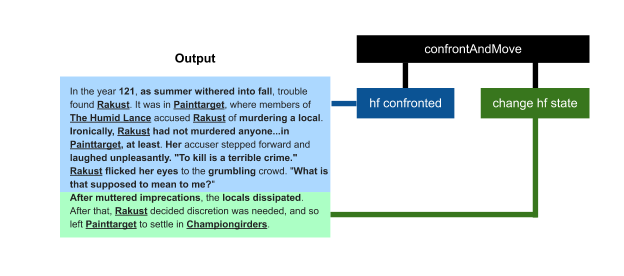
\includegraphics[width=\textwidth]{figures/4-Delve/legendswriter-diagram.png}
    \caption{Sample output from a ``bottom-up" pattern for \textit{LegendsWriter}, matching a pattern for two consecutive two events: ``hf confronted" and ``change hf state." Bold text is dynamic, underlined text denotes simulation-specific references.}
    \label{fig:legendswriter-diagram}
\end{figure}

%%%%%%%%%%%% END FIGURE %%%%%%%%%%%%%%%%%%%%%%%%%%%%%%%%

Bottom-up approaches have a higher likelihood of matching to more total events in general, as they are more granular. Similarly, this approach is more well-suited for narrativization that requires us to increment and consider events ``live", or one tick at a time, as it supports matching on only one or two events as they're added. However, its granularity also means there is a greater potential for more unforeseen juxtapositions, and bridging between those instantiations is difficult. 

Additionally, in order to apply the bottom-up approach to \textit{Delve}, we would need either a very diverse set of simulation events (which it was felt would divert too much time that could be better spent on the narrativization itself) or to author dynamic enough single-event instantiations that the output wouldn't be repetitious. It was concluded that doing that authoring work to react to context might be better served instead using the top-down approach, which as we'll see in the next section, allows more context to be layered in.

However, we will revisit the bottom-up approach in future work for \textit{Delve}, when we tackle time ticking forward as the player plays the game, creating more memories for characters. Doing so will require either adapting the top-down events in some way to fit the "live" constraints of event generation, or possibly a completely differently-designed class of events to fit the bottom-up approach. Again, to emphasize: the difference between these two approaches is not procedural or apparent on the code level, but rather wholly contained within the design of the content used by the system. The capabilities of the authoring system can facilitate either strategy.

\subparagraph{Top-Down}\label{subpar:delve-top-down}

Another story-sifting approach involves specifying longer event sequences to match. These top-down sifting patterns may contain several events in sequence to be matched, with potentially some number of allowed events in-between.

Consider a sifting pattern that covers 50 events, and also establishes some parameters or bindings for those 50 events (such as a protagonist character). When we recursively run this process for smaller groups of events within those 50, we can pass those parameters in, further contextualizing the output of those grammars. And if those patterns have matching sequences that are, say, 10 events long, when we drill down into sifting patterns that are even smaller, we pass down both the parameters from the 50-event sifting pattern, and the 10-event sifting pattern. This way, we preserve coherency in the story's structure, and can also enrich on a very granular level the per-event sifting pattern. For example, just because a character feels shy at a party, doesn't mean they have to feel shy at all subsequent parties in their life. Therefore, what we want is \textit{local consistency} and \textit{global variance}. Figure \ref{fig:legendswriter-output-tiquo} provides an example of the output from such a top-down sifting pattern in \textit{LegendsWriter}.


% \begin{quote}
%     \textbf{Tiquo}'s terrible obsession began in \textbf{71, when shadows were long and the sun red}. \textbf{He} resolved that \textbf{he} would not succumb to old age, but instead would discover the secret of immortality no matter the cost. \\
% \textbf{After mere months}, \textbf{Tiquo} found what he sought. All other avenues had been exhausted. The only remaining option was \textbf{desecration}. The temple at \textbf{Fruitthroats} was where, with reckless abandon, \textbf{Tiquo drove the priests screaming from the sanctuary and fouled the sacrament}. \\
% But \textbf{Tiquo's} actions had not gone unnoticed. The \textbf{Sunfish god Aco, arbiter of coasts, whose terrible form is worshiped by The Nation of Scribing}, had witnessed the deliberate destruction of his most holy place, and thus \textbf{enraged}, cursed \textbf{Tiquo} to the horrific form of \textbf{vampire, doomed to eternally thirst for blood}. But \textbf{Aco's} fury was \textbf{Tiquo's} gain, for \textbf{he} had seized an immortality, even though monstrous, for his own.
% \label{fig:top-down-sifting-example}
% \end{quote}
%%%%%%%% BEGIN FIGURE %%%%%%%%%%%%%%%%%%%%%%%%%%%%%%%%%

\begin{figure}
    \centering
    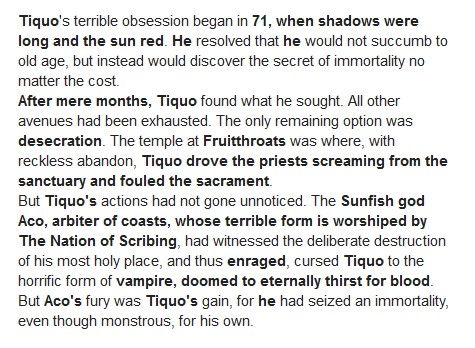
\includegraphics[width=\textwidth]{figures/4-Delve/legendswriter-output-tiquo.jpg}
    \caption{Example output from a sifting pattern with top-down approach. Bold text is dynamic.}
    \label{fig:legendswriter-output-tiquo}
\end{figure}

%%%%%%%%%%%% END FIGURE %%%%%%%%%%%%%%%%%%%%%%%%%%%%%%%%

The top-down strategy has its limitations too, however. This is because, if we used it for a simulation ticking forward in a ``live" manner, we may pre-suppose a commitment to a future event in order to match a top-level ``large time period" event, which may be invalidated by a set of effects or generated event before the pattern is matched. Put another way, it could mean that at any given point we may have one or several sifting patterns determining what a character's future holds (in an earlier \textit{Delve} prototype this was called a character’s \textit{geas} or \textit{fate}).

These issues occur from the ``liveness" of the simulation, but also because the procedures of the simulation can potentially be in conflict with the procedures of the narrativization. The top-down approach works best when the only mechanics that can influence the simulation occur within the event library. Essentially, if there are state changes that can occur that aren't accounted for by the event library, then there's a chance the game can transition to an invalid state that it can't recover from. This is because the rules governing the player's interactions may not match up exactly with the event logic's ``rules", which are mostly hand-authored and are coherent more through design convention than procedural enforcement.

For \textit{Delve}, we're not dealing with live simulation. Rather, our use-case is the initial pre-populated character histories which we want to represent as objects. For that, the desired quality for our narrativization is coherence over coverage. We want more control over multi-event character arcs---arcs driven by story logics and design more than the granularity and expressiveness of the simulation. For these reasons, we opted for the ``top-down" approach, providing its nesting context, which in turn helps control character casting and allows other references to persist across events.

To illustrate this control, imagine a collection of events encapsulating one character throwing parties and inviting other characters, then accruing favors from those friends, and finally calling in those favors later on. The difference between top-down and the bottom-up is that the top-down events can more easily enforce collections of shorter events, as shown in Figure \ref{fig:two-strategies}.

%%%%%%%% BEGIN FIGURE %%%%%%%%%%%%%%%%%%%%%%%%%%%%%%%%%

\begin{figure}
    \centering
    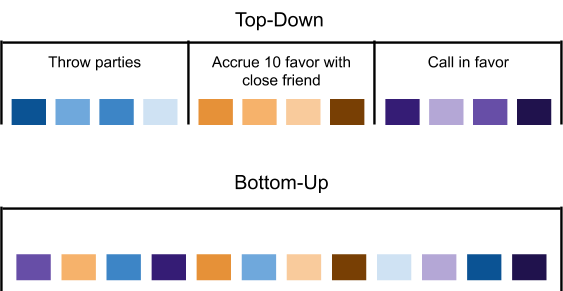
\includegraphics[width=\textwidth]{figures/4-Delve/two-strategies.png}
    \caption{Top-down approach with hierarchical scaffolds, versus bottom-up, where events are evaluated individually for pre-conditions, and surprising juxtapositions may occur, unless highly-specific preconditions are written to manually chain events.}
    \label{fig:two-strategies}
\end{figure}

%%%%%%%%%%%% END FIGURE %%%%%%%%%%%%%%%%%%%%%%%%%%%%%%%%

In contrast, in practice it would be more difficult to ensure that such specific arrangements of events happen if we generate events one at a time, then try to apply a pattern onto them. Of course one could enforce that by writing pre-condition terms to that effect, but the number of required pre-condition terms to accomplish that makes it infeasible once the number of events grows larger, and putting that number of terms on each event reduces authorial Clarity, as opposed to simply adapting a top-down approach.

\subparagraph{A Note on Hybrid Approaches}\label{subpar:a-note-on-hybrid-approaches}

Top-down approaches are good for pulling out interesting arrays of life events, and giving an over-arching shape to the character's whole life. However, given their longer sequences and higher specificity, they don’t show up for a wide variety of character lives. For example, in LegendsViewer the sifting pattern in Figure \ref{fig:legendswriter-output-tiquo} is only triggered around thirty times for a world populated by thousands of characters, containing hundreds of thousands of events. Additionally, those stories tend to look fairly similar, and so much effort must be spent to increase their surface text generativity.
 
Bottom-up grammars are good for diffusing more rendered text amongst characters. However, they require far more labor to create, given that in order to avoid sounding repetitive, they require more dynamic input. This can be solved partly with random variation of descriptions, such as the confrontation text in Figure \ref{fig:legendswriter-output}, but to truly leverage the strengths of the system it would be better if grammars vary based on parameters that are passed down to them by top-down sifting patterns. Alternatively, grammars can be made for periods of interstitial time between flags (which may contain an arbitrary number of events) which key off the highest frequency of particular events, and then output short sentences along the lines of ``the next [n] years were filled primarily with [battles], until..." The union of these two approaches is where one could potentially see both wide coverage of events, and well-formed stories emerge, though this remains in the domain of future work.

\paragraph{Generation Procedure}\label{par:delve-generation-procedure}

\textit{Delve} uses the top-down approach for these reasons, and also because simulation is not as important to the immediate research goals as generating fully fledged, rich event descriptions and evaluating the authorial burden of that. The hope is to slowly turn the dial up on the expressivity and generativity of the history generation by building out pre-conditions and effects of the events. But the most centrally important thing is the memories themselves–specifically, the semantic tags associated with them, and the breadth of generativity possible without encountering an infeasible authorial burden. If significant generativity is not accomplishable (which will only become apparent once significant content authoring has been completed) then adding simulation to the mix will be a moot point.

Event generation begins by taking all the characters, sorting them in descending order by ``power" (calculated based on pre-coded diegetic properties from the game's backstory). Then, for each character that has not yet been allocated for the current timestep, an event with satisfiable conditions is selected whose ``main character slot" can be filled by the particular character.

Each event has an Expressionist grammar key associated with it as its ``surface text." The system then calls the surface text realization system, which generates a package of potential grammar expansions, with their associated semantic tags. After this process finishes, it then passes the tags for the current ``active" state of the grammar to the ontology, to be translated into suitable nodes for memory object generation.

\paragraph{Hierarchical Nesting}\label{par:hierarchical-nesting}

The ``top-down" part of event generation is expressed and driven by the ``casting call" of each event. For each character cast, there is a paired ``bank" of other events, separated by timesteps they're valid for (see Figure \ref{fig:delve-casting-call}).

%%%%%%%% BEGIN FIGURE %%%%%%%%%%%%%%%%%%%%%%%%%%%%%%%%%

\begin{figure}
    \centering
    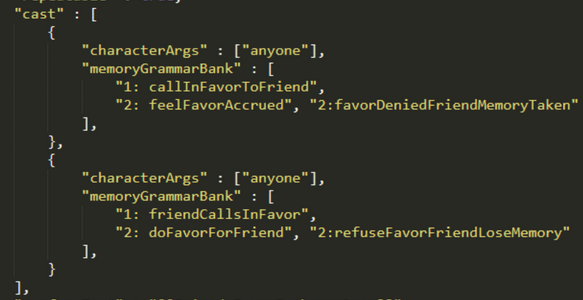
\includegraphics[width=\textwidth]{figures/4-Delve/delve-data-casting-call.png}
    \caption{A casting call for a two timestep event, where it looks for any character (``anyone") to fill its slots. Slot 1 has one event (``callInFavorToFriend") and slot 2 has two events (``feelFavorAccrued" and ``favorDeniedFriendMemoryTaken")}
    \label{fig:delve-casting-call}
\end{figure}

%%%%%%%%%%%% END FIGURE %%%%%%%%%%%%%%%%%%%%%%%%%%%%%%%%

When a multi-timestep, multi-character event is called, it proceeds through each character and expands out the events in a ``depth first"-style search, provisionally running effects as it goes. We expand in a depth-first manner because after a character’s early timestep is confirmed and run in a multi-step event, the effects are applied. If done otherwise, these applied effects could potentially change the state such that casting decisions made from an earlier state would no longer be valid. 

When the search bottoms out, it allocates all the events and runs the collected effects, then proceeds to the next character for the current timestep. If that character was allocated in the previous call (for any part of that chain) it checks the next character, and continues until it's passed through all the characters for that timestep. Then it continues to the next timestep, and repeats the same process for the events that haven’t been rendered out yet. If it turns out we can’t process the event due to the preconditions no longer being valid, we bump up the tree to the next level up, and see if we can process from there.

One of the content design implications from this approach is that, from a dramatic perspective, events need to be written with the first cast slot as the most important or central to the event. It also means that characters who are of lesser power are more likely to get drawn into events by more powerful characters (since they go first, and have the opportunity to cast lower power characters in their events).

A more in-depth discussion of \textit{Delve}'s hierarchical event nesting can be found in Section \ref{subsubsec:delve-implementation-event-generation}'s discussion of event generation. But at a high level, this event structure means we can group events together under loose categories (happyWalking and sadWalking in a memoryGrammarBank for walking) and chain them for long timesteps. You could even have just one giant event that encapsulates an entire character's life called ``tragicLife" that has 1000 timesteps, composed of 5 100-timestep ``normalLife" sub-events, followed by 3 100-timestep``wonderfulLife" sub-events, followed by 1 100-timestep ``terribleLife", and 1 100-timestep ``disastrousLife." These loose categories would have very large memoryGrammarBanks, but would allow the author to specify an overarching structure for this character’s life that is generative, but still strictly controllable. In fact, \textit{Delve} does precisely this on a code level---it starts the history simulation with a placeholder system-generated event that lasts for as long as the total history length, with a cast of all the characters, with each character containing a memoryGrammarBank consisting of all events in the library. Then it proceeds in a top-down manner, and when the process finishes, the total history has been simulated.

\paragraph{Expressionist Surface Text}\label{par:expressionist-surface-text}

\textit{Delve} uses a modified version of J Ryan's Expressionist \cite{ryan2016expressionist} (described in Section \ref{subsec:expressionist}) to generate surface text, by expanding event description grammars. One key difference from the default implementation of Expressionist is that when content requests are sent to \textit{Delve}'s Productionist system (which is paired with the Expressionist system) they specify a ``root symbol" to begin expanding from (the memory in question's root grammar). This allows us to author and share grammars between memories, but without the worry that we may inadvertently start with the wrong initial grammar. Alternatively, we could tag each non-terminal with a ``system tag" containing the memory ID, but this would run into other issues down the road when the grammars are semantically optimized by Reductionist.

While from a verification standpoint it's somewhat nightmarish, it would also be theoretically trivial to attach effects to Expressionist non-terminals as plaintext tags, using a domain specific language similar or identical to the one used to write event effects. Such an ``effect tag", like ``$<$char1$>$ anger +1", could allow us to get more fine-grained effects, that have a direct tie-in to the text on a more granular level than the entire event. However, there are potential fallout implications for that (especially given that the main player interaction is switching between these non-terminals for character memory interaction!) that relegate that capability to future experimentation.

\subsubsection{Memory Palace Generation}\label{subsubsec:memory-palace-generation}

Once the historical events are generated, and their semantic tagsets known, it's possible to turn them into memory objects and place them within a memory palace. But before we do that, we need to first create a memory palace---a navigable 3D space. 

Currently the procedures for creating a memory palace are somewhat provisional, enough to allow basic functionality. Planned future work is to add more features to this as needed to increase expressiveness of both the memory objects, and the actions players can take with them in relation to the palace itself, not just on an object property basis.

We want to be able to make use of different levels of specificity when grounding out memory semantic tags into physical assets. It's advantageous for us to group objects under some sort of common concept node, and use a physical characteristic or asset to unify them. For one, it helps generalize properties to increase the chances the player will remember and understand them. For example, having five objects next to a furry rug is less cognitive overhead than, say, coming up with five or six different instantiations to symbolize the concept ``cat." Therefore, the system attempts to group memories together in order to represent common memory semantic tags, and use resulting representation strategies that can apply to multiple objects with one instantiation. Once it finds common semantic tags, it has two methods it can use to ground them out.

%%%%%%%% BEGIN FIGURE %%%%%%%%%%%%%%%%%%%%%%%%%%%%%%%%%

\begin{figure}
    \centering
    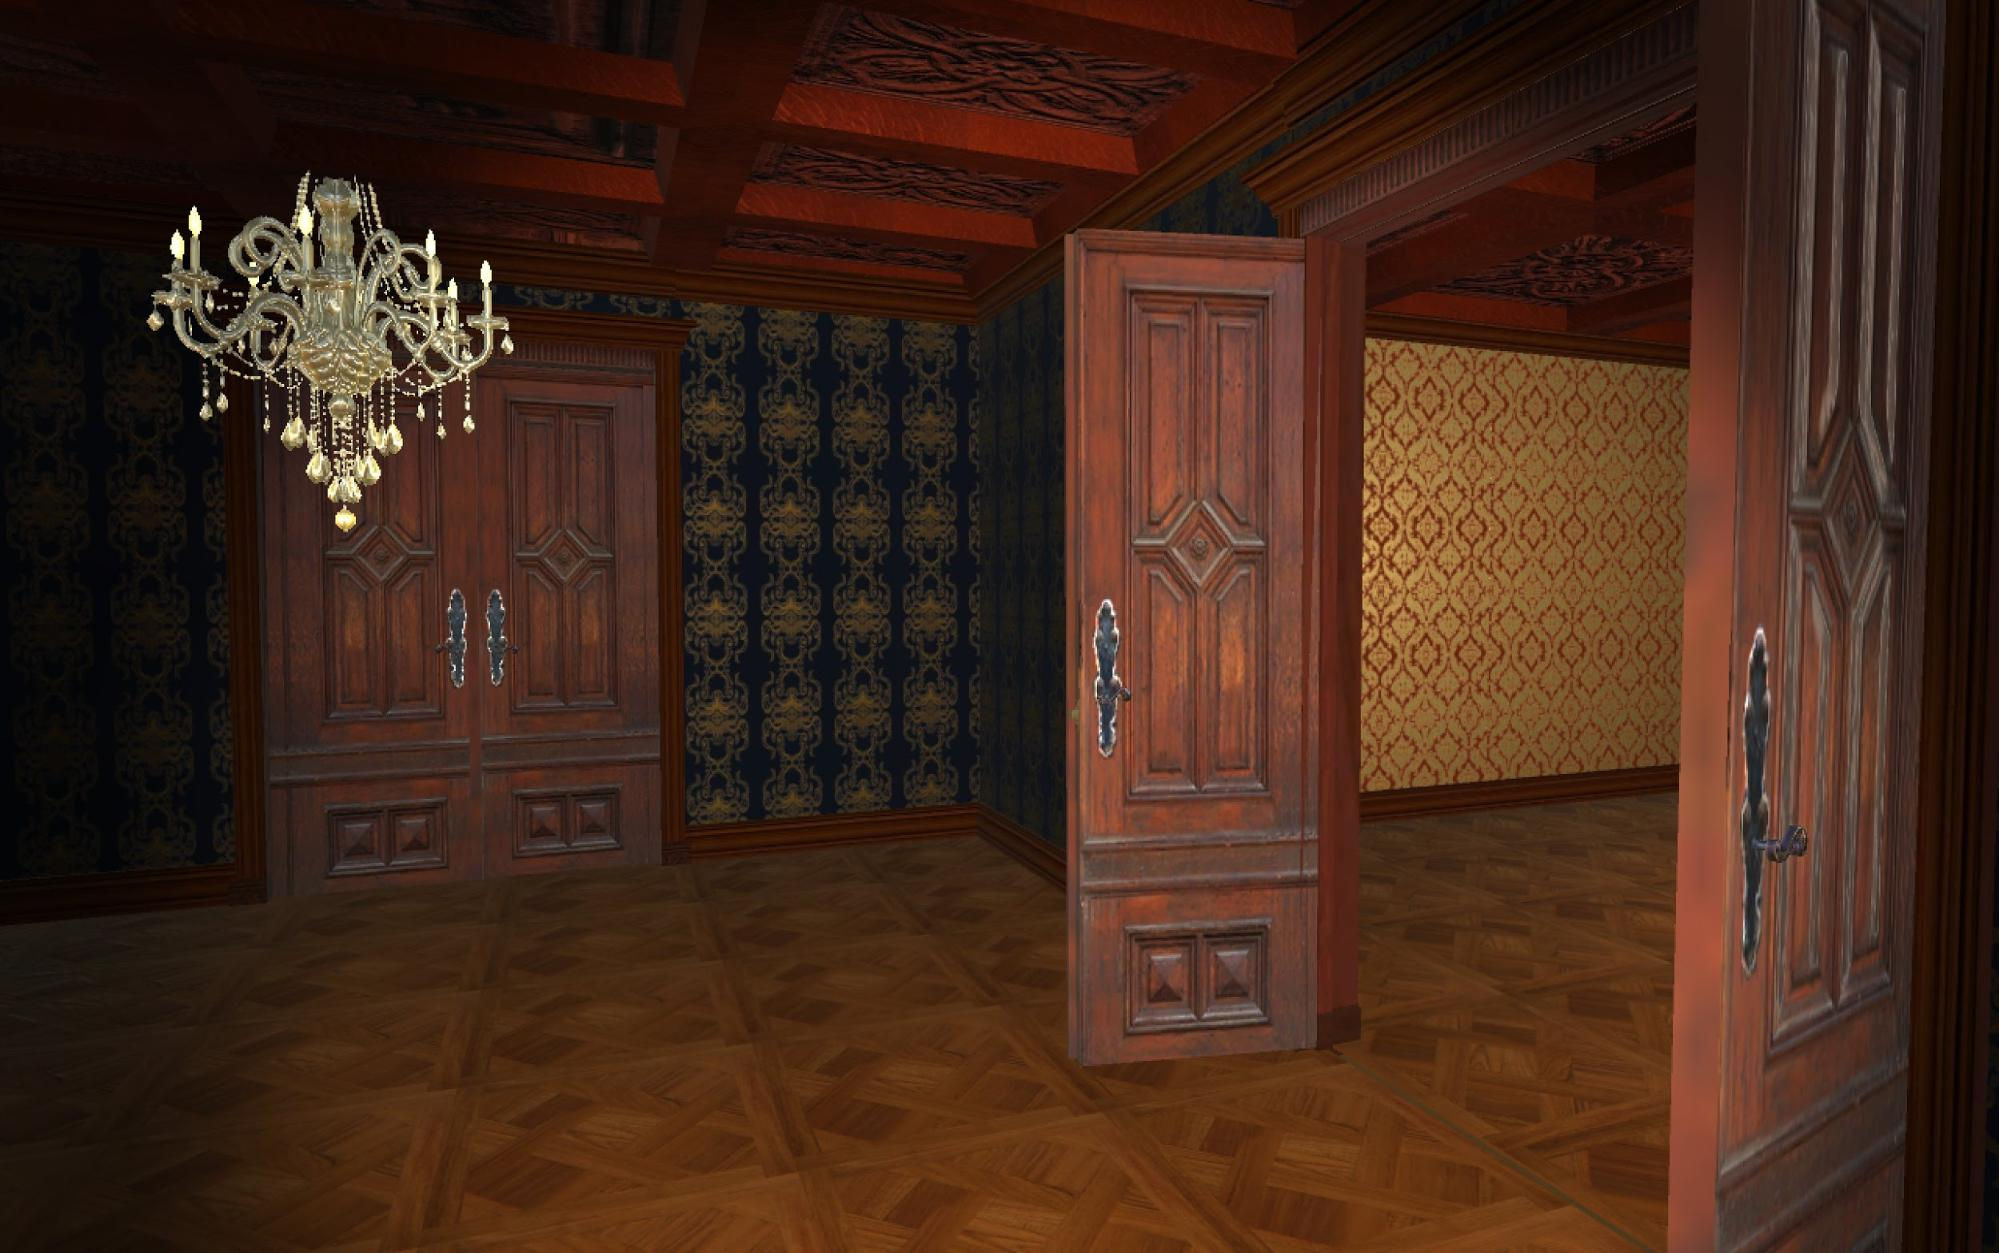
\includegraphics[width=\textwidth]{figures/4-Delve/room.jpg}
    \caption{Two rooms in \textit{Delve} with two different ``room-level" tags driving wallpaper instantiation (here, blue wallpaper for ``water" and gold wallpaper for ``wealth")}
    \label{fig:delve-room}
\end{figure}

%%%%%%%%%%%% END FIGURE %%%%%%%%%%%%%%%%%%%%%%%%%%%%%%%%

The largest-grained method is grouping into a common room. The system queries the Substrate (the game ontology) to see if there are any ``room-level" nodes reachable from the semantic tag's concept. Currently, the only room-level nodes are ones which control the wallpaper on the walls of the room. So for example, five memories with the semantic tag ``wealth" could be placed into a room with golden wallpaper (Figure \ref{fig:delve-room}).

If there aren't enough common semantic tags to group by room, but enough to have a group \textit{within} a room (a configurable variable left to artistic license) a "room location" method is used. For example, a fireplace may be added to a room, and objects placed near it that have the semantic tag "happy", which is connected metaphorically to "warm." This strategy allows memories not containing that semantic tag to still be represented in the room, as long as they are away from the fireplace. One issue this creates is that objects which are movable in a room with, for example, the "happy fireplace", will need a semantic tag state such that "happy" is part of it, in case the player moves the object next to the fireplace. This problem is one of the authorial warning bells that is gone into in more depth in Section \ref{subsubsec:delve-explorability} on Explorability.

Once we have a room with objects, we also need to be able to get to different rooms. This also is still a fairly nascent system, but there are two methods that were experimented with. One was to place a symbolic object (such as a statue) near the door to symbolize the room that door led to. This approach was abandoned, because it was too easy to confuse those objects with memory objects, and their lack of interactivity was confusing. For now, rooms are connected to each other through a simple door, or they can have an interstitial hallway. The hallway, if connecting between two rooms with a wallpaper-grouping tag active, transitions from one wallpaper to another for the respective doors at each end.

Hallways also enabled us to make use of an exploratory concept node realization method: floorplan layout. There are future plans to make much more use of this, but for now the sole method is that a room-level concept node of ``lonely" will force a room to be connected via only one door to other rooms, through a very long hallway. In general we don't concern ourselves with floorplan layout for the same reason we aren't concerned with consistent mapping in land generation: there is existing research tackling such issues (such as integrated semantic coordination \cite{semantic_building}, graph grammars \cite{bidarra_designing}, and other approaches) and it is secondary to our primary focus of dynamic memory generation and placement.

Lastly (though this exists only on a code level with text realization, and cannot be seen directly in the Unity prototype) an external facade is generated from looking at which semantic tags the character has the most of, and can make a simple text description from that. For example, a character whose highest recurring semantic tags are ``stubborn" and ``haughty" might generate a facade description of a ``front door that is stubbornly iron", and ``a roof that is haughtily steep." This is intended at some point in the future to provide players with a hint of what kind of character they are interacting with before they enter the palace, though all of the systems are in place to drive that pipeline once it becomes a priority.

\subsection{Implementation Details}\label{subsec:delve-implementation-details}

While StoryAssembler was abstracted out into a stand-alone library from its initial implementation in \textit{Emma's Journey}, the systems of \textit{Delve} (like \textit{Ice-Bound}) are currently inextricable from their in-game implementation. There are, however, some details specific to the implementation that bear mentioning, that have concrete implications for the systems' more abstract details mentioned in the previous section.

\subsubsection{Land Generation}\label{subsubsec:delve-implementation-land-generation}

Land generation, as mentioned in the previous section, is fairly nascent, so the systems to generate them are not complex or nuanced. There are a set number of ``types" of land, and for each one a list of landscape props, along with a weight. The system first picks a type of land to generate, then places a certain number of props within it, using the weight to drive the random selection. This could be easily expanded upon to provide more diverse land types and starting props, but the current implementation has simply three types (forest, mountain, and plains) with various concentrations of six nature prop types (tree, bush, stream, rock, flower, grass). Events are planned at some future date to operate on props to form the beginnings of houses or even cities. One can imagine, for example, sequences of events that require some number of tree props as cast, then forms a small house from them, which a character then lives in.

\subsubsection{Character Generation}\label{subsubsec:delve-implementation-character-generation}

Most of a character's qualities derive from the events comprising their timeline, and the events themselves are the main focus of this endeavor. Thus, the initial character generation is fairly simple. An initial weight in a few concepts is randomly given, and a few relationships to other characters are given, with a randomly selected concept. This allows characters to pass initial casting checks for events that require a supporting character with some sort of relationship to them.

\subsubsection{Event Generation}\label{subsubsec:delve-implementation-event-generation}

%%%%%%%% BEGIN FIGURE %%%%%%%%%%%%%%%%%%%%%%%%%%%%%%%%%

\begin{figure}
    \centering
    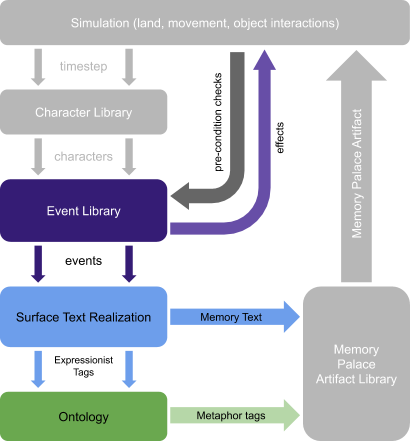
\includegraphics[width=10cm]{figures/4-Delve/delve-diagram-highlight.png}
    \caption{Highlighted sections of \textit{Delve}'s original execution flow handling event generation.}
    \label{fig:diagram-highlighted}
\end{figure}

%%%%%%%%%%%% END FIGURE %%%%%%%%%%%%%%%%%%%%%%%%%%%%%%%%

Events and their generation are the core focus of \textit{Delve}. As mentioned in Section \ref{subpar:delve-top-down}, \textit{Delve} uses a ``top-down" approach, passing down context from parent events, which are recursively called from the initial ``virtual event" that begins generation and encapsulates the length of the entire history for every character. Events have three categories of components, which we'll take in turn: pre-conditions / effects, surface text, and casting / recursion.

\paragraph{Pre-conditions and Effects}\label{par:delve-pre-conditions-and-effects}

\textit{Delve}, like \textit{Ice-Bound} and StoryAssembler works, uses a simple DSL for preconditions and effects. In terms of preconditions, it is of comparable simplicity, using a blackboard which can be populated by strings, integers, or float values.

Effects, however, are more complex. This grew out of the desire to build in expressivity that could be leveraged later on, to create events that proceed in a more ``live" fashion after the initial generation has happened (perhaps in a more ``bottom up" authoring approach). As such, we wanted to put in hooks for some ``exemplar" cases, to see how they felt from a content authoring perspective, and whether they could be sustainably implemented when the time came. While that evaluation is still to be done, the initial implementation was completed for test purposes. A good example of such a test effect is ``eat([random prop] withinDistance\_0 [cast\_0]) : 1", which translates to ``on the first timestep of this event, run the function eat(), passing it a random object of type Prop that is in the same area of the character cast in the first slot of this event." In this case, the eat() function is defined in a C\# library (and thus has access to all data or functions of the game) and consumes a passed in object, while giving its highest ranking concept quality (say, ``tree") to the consumer. Thus, this effect would have the effect of increasing a character's ``tree" quality by 1, and deleting a tree prop from the land the character occupied.

\paragraph{Surface Text}\label{par:delve-implementation-surface-text}

%%%%%%%% BEGIN FIGURE %%%%%%%%%%%%%%%%%%%%%%%%%%%%%%%%%

\begin{figure}
    \centering
    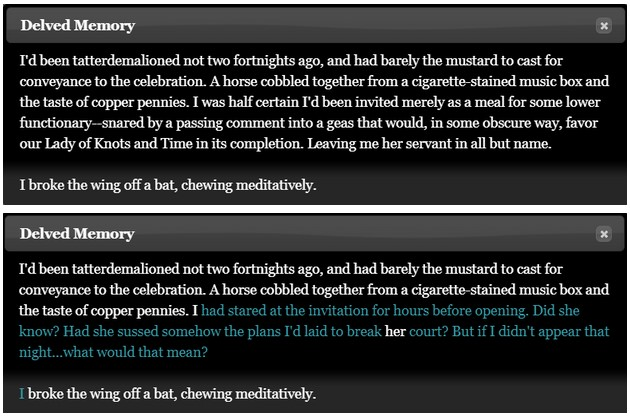
\includegraphics[width=12cm]{figures/4-Delve/memory-detail-changed.jpg}
    \caption{An example of a changed memory. In the top version, the semantic tags ``travel, poor, horse, danger" are active. In the bottom, the ``danger" tag has been replaced with a ``rebel" tag.}
    \label{fig:memory-detail-changed}
\end{figure}

%%%%%%%%%%%% END FIGURE %%%%%%%%%%%%%%%%%%%%%%%%%%%%%%%%

In terms of pragmatic implementation, character memories consist of one or two paragraphs of text (Figure \ref{fig:memory-detail-changed}). This text is displayed to the player when they left-click on a memory object. The text changes when transformations are applied to the object, which in this initial implementation consists of a ``transmute" action triggered by right-clicking on the object. The text that changes is highlighted in blue, in order to help accent how it has changed. 

\paragraph{Casting / Event recursion}\label{par:delve-casting-event-recursion}

The heart of \textit{Delve}'s complexity, its affordance and challenge, is its hierarchical recursive nesting. This is expressed in events through the ``cast" call, due to the character-centric focus of the narrative and system.

``Cast" is an array, and can be any number of character objects. For clarity, we'll refer to the first character in this array as the \textit{lead}. Each cast character has their own ``characterArgs" which, like \textit{Ice-Bound} and StoryAssembler works, can be either explicit by ID, filled by any character possessing a certain quality, or the all-encompassing ``anyone."

Each character cast also has a ``memoryGrammarBank." This is an array of tuples: a timestep index, and a paired event id. This makes events a tree structure, which can reify out or potentially even loop back on itself (which requires careful use of effects and preconditions to avoid infinite recursion). For each timestep of the event, it iterates over each cast member's ``memoryGrammarBank" (starting with the lead) and chooses a valid one to process (based on whether the pre-conditions are valid, and it can be cast in turn). Currently, it's designed to favor events whose timesteps are largest (while still less than or equal to the remaining time of the parent event) and favors events which can themselves be cast with the characters cast in the parent. Failing that, it proceeds to try to cast characters that are lower-status than the lead, and who have a similar Dominion (highest ranking Substrate concept node) to the lead character.

The essence of the casting proceeding from lead, and organized by decreasing power, is what gives this recursion its hierarchical nature. This was favored because the fictional world of \textit{Delve}, that of a faerie court, is one which is strictly (if nonsensically) hierarchical. Therefore, the predilections of the content planned for this experience will be supported by this hierarchical approach. Because the events ground out depth-first, there's a higher chance a more powerful character will be calling the shots by allocating the event a weaker character enacts for that. 

%%%%%%%% BEGIN FIGURE %%%%%%%%%%%%%%%%%%%%%%%%%%%%%%%%%

\begin{figure}
    \centering
    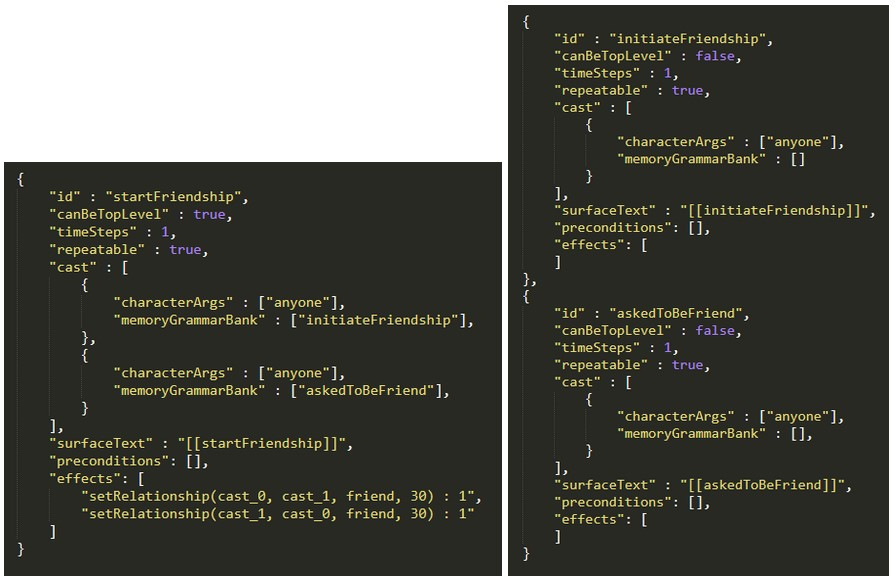
\includegraphics[width=\textwidth]{figures/4-Delve/delve-data-one-step-event-sequence.jpg}
    \caption{An example of a one-step nesting event sequence. One character will have the event ``initiateFriendship" added to their memory palace, and one will have ``askedToBeFriend" added to theirs. Both characters will have the ``startFriendship" event as a reference, but the ``startFriendship" grammar is not associated with a given memory object.}
    \label{fig:one-step-event-sequence}
\end{figure}

%%%%%%%%%%%% END FIGURE %%%%%%%%%%%%%%%%%%%%%%%%%%%%%%%%

It's best perhaps to illustrate through a concrete example (Figure \ref{fig:one-step-event-sequence}). Take a (relatively) simple, one-timestep event: ``startFriendship." This event has two cast slots. Let's say the first one is filled by char1 (who has higher power), the second by char2. The startFriendship event can call only one potential event for char1 (initiateFriendship) and one for char2 (askedToBeFriend). It calls each in turn, which have no ids in their respective memoryGrammarBanks. Because of this, the system knows these are leaf events, and assigns them as the events in each respective character's timeline.

The ``startFriendship" event that started it off also has a surfaceText grammar, even though only leaf nodes can be associated with memory palace objects. However, one use for this text (at least in experimenting with prototypes) was to provide an ``objective" timeline. Because ``startFriendship" is called as a top-level event, its description is added to this log. There aren't any current plans to provide such a log to the player, but it remains an expressive affordance of the system.

We also see two effects run in ``startFriendship", which set the ``friend" relationship of char1 to char2 to 30, and vice versa. Again, relationship concepts are tied into the ontology; there is no fixed set of concepts for social relationships (a character could, for example, have a positive ``pie" relationship with a baker). This is still a fairly nascent system, so no rigorous restraints have been put on the ontology, only affordances that, for now, will rely on authoring conventions to keep consistent.

%%%%%%%% BEGIN FIGURE %%%%%%%%%%%%%%%%%%%%%%%%%%%%%%%%%

\begin{figure}
    \centering
    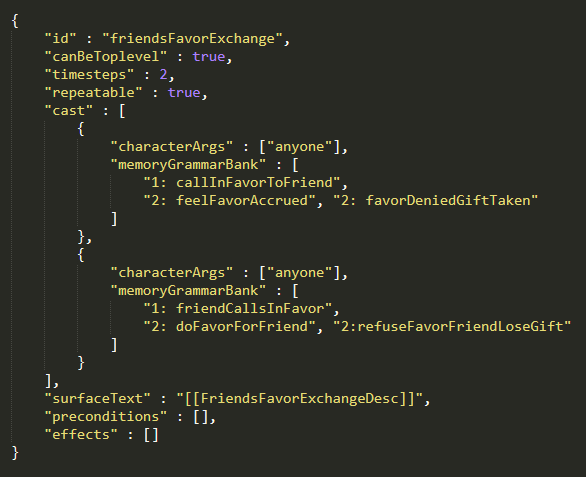
\includegraphics[width=\textwidth]{figures/4-Delve/delve-complex-event.png}
    \caption{A slightly more complex event. This one demonstrates a character calling in a ``favor" to a friend, which can be either honored or refused (the latter resulting in the other character's gift being taken).}
    \label{fig:complex-event-sequence}
\end{figure}

%%%%%%%%%%%% END FIGURE %%%%%%%%%%%%%%%%%%%%%%%%%%%%%%%%

Let's look at one more concrete example of a slightly more complex event (Figure \ref{fig:complex-event-sequence}). This is a similar structure (two characters, two timesteps, one step of recursion) of an event where one character asks for a favor from the other, and the favor is granted or denied (the six leaf events are not shown, for space reasons). In this case we see the first character slot will always first have ``callInFavorToFriend" as their first event, but has two potential events for timestep two. If the ``feelFavorAccrued" preconditions are met, it will be chosen as the second event. This has an effect which chains with the preconditions for the subsequent events for char2, which chooses (in this case) ``doFavorForFriend." Thus, we have char1, with the event progression "callInFavorToFriend -> feelFavorAccrued" and char2, with event progression ``friendCallsInFavor -> doFavorForFriend."

\subsubsection{Memory Palace Generation}\label{subsubsec:delve-implementation-memory-palace-generation}

Now that we've talked in technical detail about how the textual data is generated for memories, we can talk about their 3D instantiations. We'll first discuss the ontology used to tie the text to the realization systems, then talk about the generation of the palace itself---consisting of both layout and room generation---finishing with how the memory objects themselves are generated.

\paragraph{The Substrate}\label{par:delve-implementation-the-substrate}

The data graph that provides connective coordination between these different systems (called the Substrate) is a simple ontology consisting of a few node and connection types (Figure \ref{fig:substrate-ontology}). Because the focus on this project was more on the generative space of the narrative this type of system could afford, the Substrate is not as systemically rigorous as those like ConceptNet \cite{liu2004conceptnet} or CyC \cite{cyc}, or as conceptually nuanced as the ones underlying works like Zhu's \textit{Riu} \cite{zhu2010story}. However it does provide a vital function, in that it supplies a structured and unified system of content tagging, to be leveraged by the game systems in a cohesive manner. Rather than focus on adapting an existing ontology like ConceptNet, or otherwise process material into ontological relations, we wanted to treat data entry to the Substrate as a creative process of association, and see where the initial approach led us.

%%%%%%%% BEGIN FIGURE %%%%%%%%%%%%%%%%%%%%%%%%%%%%%%%%%

\begin{figure}
    \centering
    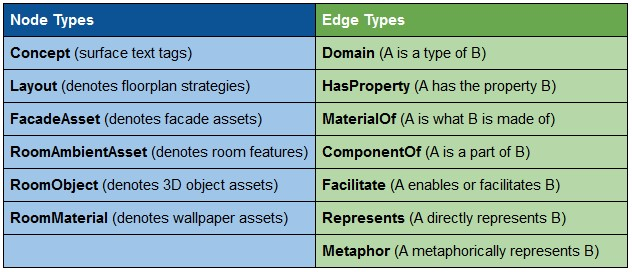
\includegraphics[width=\textwidth]{figures/4-Delve/substrate-ontology.jpg}
    \caption{The node and edge types of the Substrate.}
    \label{fig:substrate-ontology}
\end{figure}

%%%%%%%%%%%% END FIGURE %%%%%%%%%%%%%%%%%%%%%%%%%%%%%%%%

When the system conducts various queries to instantiate content, it is provided a starting point, a target node type, a ``whitelist" of valid edge types, and a maximum number of allowed steps. It then runs a simple search to return valid nodes. Each given node type is its own class with its own member properties, which assist in instantiation.

While further developing the complexity of the Substrate, perhaps to assist in more sophisticated metaphoric or poetic reasoning, is certainly on the list of future developments, we found the initial capabilities of the system sufficient to start drafting content, so that we could begin to explore the content dynamics of textual memories instantiated in a 3D environment.

\paragraph{Layout Generation}\label{par:delve-implementation-layout-generation}

As mentioned earlier, the domain of procedural building layout generation is a well-developed research area with many different techniques, even ones leveraging conceptual networks for semantic coordination \cite{semantic_building}, but is not our particular focus at this time. We are more concerned with the authoring challenge of objects when situated within rooms, and how that can be changed. That said, some hooks were put in for some initial expressive leverage. The ``layout" nodes in the Substrate denote classes of approaches for connecting rooms to each other. Future work is planned for this to encapsulate different floorplan techniques, but for now (as mentioned in Section \ref{subsubsec:memory-palace-generation}) an initial singular affordance was put in to express the concept ``lonely": an especially long hallway isolating the room from others. Connections between rooms can be either immediate (a door on a shared wall) or through a hallway.

We sidestep entirely the problems of layout generation by leaning on the fiction of the world. Because the memory palace is within the mind of the character, we can violate the normal laws of physical space. Simply put: doors close automatically behind players, and rooms are only made visible in the game when their door opens for the player to pass through. Thus, we only have to have a central room (which the player occupies) and any connecting rooms activated at a given time. This affords disorienting and dream-like logic (such as taking four right-angle doorways and not ending up where one started, but in a different room altogether) which suits the fiction, in addition to setting us free from some of the attendant thorny issues that require layout generation algorithms in the first place. Thus, a floorplan for \textit{Delve} simply consists of a list of rooms with some number of memories allocated per-room (by common concept if possible), and connection types.

\paragraph{Room Generation}\label{par:delve-implementation-room-generation}

Having created a floorplan, room generation can now occur. A simple square baseline room is created. Then, the system checks if there are any semantic tags common to all memories grouped in the room. If so, it then checks to see if there are any ``RoomMaterial" nodes it can reach from that semantic tag's correlating concept node in the Substrate, and if so, modifies the wallpaper.

Then, it checks to see if there are any groups of memories with common semantic tags. If so, it then searches to see if there are any ``RoomAmbientAsset" nodes that can be reached from the semantic tag's correlating concept node, and if so, instantiates them using that reference, and places the memories close to them. For any memories that are left, it places them (for now) randomly throughout the room.

In the future, determining more room-level and ambient features a room may contain will be a key feature of expressivity for \textit{Delve}, as one of the key player verbs will be moving objects around the room, or perhaps even between rooms. Therefore, pushing the expressivity of ambient room assets such that objects can be creatively explored by moving them around will be a future focus.

\paragraph{Object Generation}\label{par:delve-implementation-object-generation}

%%%%%%%% BEGIN FIGURE %%%%%%%%%%%%%%%%%%%%%%%%%%%%%%%%%

\begin{figure}
    \centering
    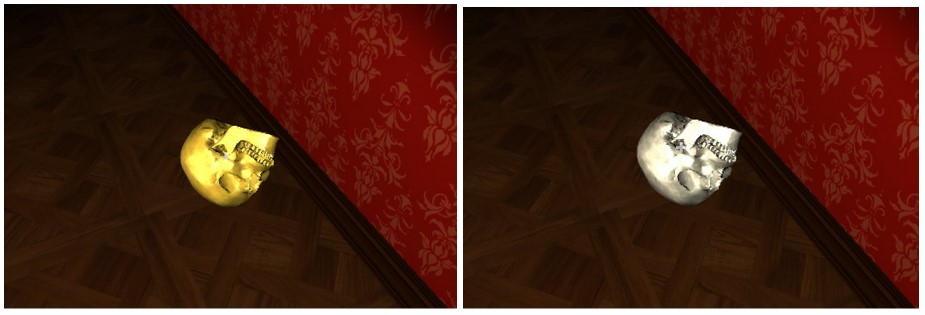
\includegraphics[width=\textwidth]{figures/4-Delve/transmutation.jpg}
    \caption{A sample memory object, before and after it's been transmuted and its memory altered.}
    \label{fig:transmutation}
\end{figure}

%%%%%%%%%%%% END FIGURE %%%%%%%%%%%%%%%%%%%%%%%%%%%%%%%%

Once the rooms have been created, and it's known which semantic tags have been allocated due to floorplan or ambient room feature, we can now at last create memory objects.

Memory objects, because of their changeable nature, are collections of configurations. For each memory, the object manager system comes up with a series of configurations which can express the semantic tags of the referenced memory's complete tag dataset, whether currently active or inactive. Object configurations are given an ``expressivity score" based on how many of their properties directly map to semantic tag concept nodes (mostly through the ``hasProperty" and ``metaphor" Substrate edges).

After this has been calculated, the current active tagset's object configuration is chosen, and the object is instantiated in the scene. When the player interacts with the object (currently limited to ``transmutation", which changes the object material) an object configuration is chosen with a different material mapping, and the memory semantic tags associated with that config are sent as an Expressionist request, so that the memory text is updated accordingly.

\subsection{Content Creation for \textit{Delve}}\label{subsec:content-creation-for-delve}

Content creation for \textit{Delve} is the most complex of the three projects, due to the interconnectedness of the systems. Broadly speaking, it consists of four steps: 
\newline
\begin{enumerate}
    \item authoring event data
    \item writing the generative Expressionist grammar for event surface text
    \item semantically tagging the grammar and adding corresponding concept nodes and connecting edges into the ontology
    \item adding any necessary 3D assets required to instantiate the memory
\end{enumerate}

We will take each of these in turn, talking more now about the technical and design details involved in the task of creating content for this experience.

\subsubsection{Authoring Event Data}\label{subsubsec:delve-authoring-event-data}

%%%%%%%% BEGIN FIGURE %%%%%%%%%%%%%%%%%%%%%%%%%%%%%%%%%

\begin{figure}
    \centering
    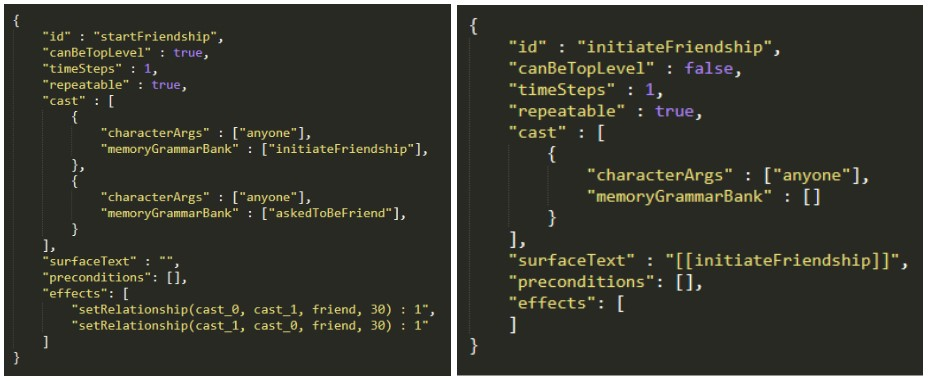
\includegraphics[width=\textwidth]{figures/4-Delve/structural-and-descriptive-events.jpg}
    \caption{Two events for \textit{Delve}. The one on the left (``startFriendship") is a structural event, with no content of its own, but establishes banks of sub-events for characters, and runs some effects (in this case making the characters friends). The right event is a descriptive event, which has the manipulable text (initiateFriendship).}
    \label{fig:structural-and-descriptive-events}
\end{figure}

%%%%%%%%%%%% END FIGURE %%%%%%%%%%%%%%%%%%%%%%%%%%%%%%%%

The first task when authoring content is to put in the event data structure. This contains the pre-conditions and effects that are simulation-facing, and also contains references to the grammars that will generate the surface text of the event for the character.

\textit{Delve}'s systems, like StoryAssembler, can enable a broad range of narrative dynamics. Therefore, a critical first step before simply creating events is establishing patterns for what types of events need to be authored, and how they work as a whole. Therefore, some initial points must be made about design.

There are actually two kinds of \textit{Delve} events, which fall out of their recursive dynamics: \textit{structural}, and \textit{descriptive} (Figure \ref{fig:structural-and-descriptive-events}). \textit{Structural} events set up the structure of the timesteps they encapsulate, by sub-dividing them into discrete segments per-character. They pass in their contextual effects to those sub-event calls, and establish casting preferences. \textit{Descriptive} events deliver the surface text.

This suggests some initial authoring patterns to investigate, as---because the content to date has been mostly proof of concept as the systems were being built out---many of these patterns are speculative. Future work will need to be done to see how their dynamics play out, and how implementation of such patterns at scale for an interactive experience intersects with the authorial leverage challenges of the system, which will be elaborated on in Section \ref{subsec:delve-authorability}'s discussion of Authorability.

These provisional patterns operate in the same spirit as StoryAssembler authoring patterns. They're not as ``story dynamic specific" as Ashwell's ``Standard Patterns in Choice-Based Games" \cite{ashwell_choice} or Short's adaptation of those patterns to storylet-based games \cite{short_storylets}, but they do provide some broad (or extreme) structural examples that we can use to see what content authoring dynamics result. Additionally, there's obviously a spectrum between large timestep events versus small, but we'll talk about larger timestep events, in order to make them more illustrative.

%%%%%%%% BEGIN FIGURE %%%%%%%%%%%%%%%%%%%%%%%%%%%%%%%%%

\begin{figure}
    \centering
    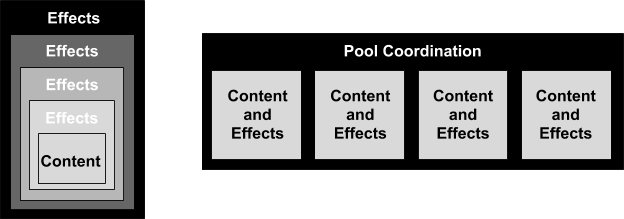
\includegraphics[width=\textwidth]{figures/4-Delve/authoring-patterns.png}
    \caption{Two broad patterns of thinking about authoring, shown with five events each: the ``chain" (left) and the ``comb" (right).}
    \label{fig:delve-authoring-patterns}
\end{figure}

%%%%%%%%%%%% END FIGURE %%%%%%%%%%%%%%%%%%%%%%%%%%%%%%%%

\paragraph{The Chain}\label{par:delve-the-chain}

``The Chain" (to the left in Figure \ref{fig:delve-authoring-patterns}) is a pattern that falls out from pushing combinatorics on the depth of the recursion for content. In an extreme version, one could imagine this as four purely structural events, with the same number of cast in each, with one descriptive event at the end of the recursion. The expressiveness would rise from the flexibility of the descriptive event, which would need to operate on the possible combinatorics of effects or blackboard context variables coming from different calls from subsequent parent events. One could imagine, for example, setting up five blackboard variables: valance, place, time, and main character mood. Thus, we could end up with a library (as long as the descriptive event at the end could express it) that could give us a ``[sad] party at a [pond] at [twilight] where the character is [happy]", or a ``[happy] party at a [tavern] at [noon] where the character is [sad]." The pattern here would be geared towards giving us many different types of parties, through the use of effects and blackboard state.

\paragraph{The Comb}\label{par:delve-the-comb}

``The Comb" (to the right in Figure \ref{fig:delve-authoring-patterns}) is a pattern that pushes combinatorics on the ordering of events. There is only one structural event, but the complexity arises from which events are specified in the timestep pools, and the checking of pre-conditions for their selection. This would be a good pattern for modifying a quality over time, and brings to mind the authoring emphasis in \textit{Emma's Journey}, which was about having many individual fragments with effects that would make progress over several choice points to change a blackboard variable to a certain value. This would sacrifice richer individual context combinatorics in favor of showing shallower but consistent change over time (such as increasing and decreasing ``tension" or ``friendship").

\paragraph{Casting Call}\label{par:delve-casting-call}

%%%%%%%% BEGIN FIGURE %%%%%%%%%%%%%%%%%%%%%%%%%%%%%%%%%

\begin{figure}
    \centering
    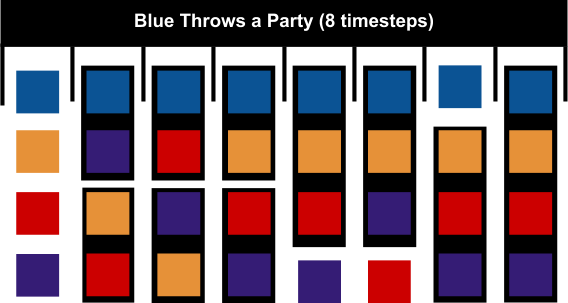
\includegraphics[width=\textwidth]{figures/4-Delve/comb-chain.png}
    \caption{A more complex pattern pushing combinatorics on character casting.}
    \label{fig:comb-chain}
\end{figure}

%%%%%%%%%%%% END FIGURE %%%%%%%%%%%%%%%%%%%%%%%%%%%%%%%%

This isn't to say that previous two patterns are exclusive, but rather where we want to spend an (assumedly) finite amount of effort per content group. However, we've pushed combinatorics on one of the casting sub-arrays (memoryGrammarBank) in two ways, so why not the other: characterArgs? This leads us to the Casting Call pattern, which is more complex to show, but nonetheless has some interesting implications.

Figure \ref{fig:comb-chain} shows an example using this pattern, where black boxes are structural events, and colored boxes are descriptive events for given characters. One could imagine a library of structural events: one eight timesteps long with four casting slots, and subsequent one timestep events with four, three, and two casting slots. These could be combined in different ways (as shown in the diagram) to give us further ``chain-like" context depth, pushing complexity rather on character casting requirements. The most obvious cast filtering method is to use the dominant qualities of said characters (their Domains). This type of approach would therefore prioritize the qualities of the characters as the point driving the casting combinatorics. The descriptive events in this case would need to emphasize those qualities in the surface text.

\subsubsection{Writing the Generative Grammars}\label{subsubsec:delve-writing-the-generative-grammars}

The surface text of events in \textit{Delve} is generated from Expressionist grammars. Expressionist, as detailed in Section \ref{subsec:expressionist}, is a system developed by J. Ryan that allows the creation of semantically tagged output, similar in function to that of attribute grammars, with the difference that tags are on non-terminal symbols, not production rules \cite{ryan2016expressionist}. The data can be queried to produce grammar expansions that require certain terms, prohibit certain terms, or even ``prefer" certain terms via a simple scoring metric (although that is an affordance reserved for future authoring).

There are at least two ways we can think about the combinatorics when creating surface text in Expressionist. A useful comparison can be made to writing event and ending cards for \textit{Ice-Bound}. One strategy is to focus on \textit{narrative variation}. This is more in line with the type of combinatorics that arose from combinations of different \textit{Ice-Bound} symbols giving rise to different events. This would ground out in such a way that one Expressionist grammar for, say, a party would need to encapsulate meaningfully different types of party memories, such as ``a party where I saw someone murdered" or ``a party where I met my true love." Hypothetically speaking (since content authoring is still provisional) one could imagine that a room filled with such objects would potentially have wildly different character narratives, depending on their configuration.

Alternatively, we could author with \textit{surface text variation}. For this, we consider surface text as having the same narrative impact for a character's life regardless of which combinations are active, but the specifics (which may be poignant, but not enough to change the overall plot) can change. This is similar to the ``shimmer text" of \textit{Ice-Bound}, which was sections of sentences that would shimmer and flash between different options, and needed to be ``resolved" by the player by tapping them, and cycling between the options until they picked one. This proved an effective way to allow the player more bespoke customization that wouldn't increase the complexity of our combinatorial considerations. It also provided a handy stand-in for when we wanted to be specific about a certain thing in an event or ending, but couldn't guarantee the activated symbols would have introduced it properly. Thus, instead of adding some sort of state setting and checking, we would instead make all options of the grammar available, and put the task to the reader to resolve. Similarly, one could imagine a room full of memory objects which can be moved around and their memory text semantic tags changed, but the character’s core story never being modified. We would shy away from the troubles of meaningful combinatoric variation, in exchange perhaps for an increase in legibility (or at least, less chance of paradox) and a willingness for the player to engage in more ``sculptural" gameplay, though those changes would mean less overall.

\subsubsection{Tags and 3D Assets}\label{subsubsec:delve-tags-and-3d-assets}

%%GDoc comments%%
The two previous modes assume a standpoint of text leading to object affordance. That is, we're talking about the breadth of variation, but not so much the object affordances. Another potential avenue for authoring content in \textit{Delve} would be to instead map out the Substrate concept nodes and the object affordances, develop a robust amount of corresponding semantic tags such that objects can be changed, moved around, etc., and then revisit the memory authoring only then. This approach might make the authoring task resemble more the stage of \textit{Ice-Bound} where we used our tools to inform what content we should author next (discussed in Section \ref{par:icebound-design-goals}). Like Calvino's \textit{Mr. Palomar} or Perec's \textit{Life: A User's Manual}, we would then tackle memory authoring knowing the thematic tree structure we would need to satisfy, and constrain the writing primarily to the vagaries of the approach, not vice versa.
%%GDoc comments%%

These approaches will be investigated in the future as content authoring strategies, in order to determine where the expressive focus of the content and system should lie (a decision borne by pragmatics, but also artistic choice). This sort of interplay between Traversability and Authorability will be expanded upon in their respective upcoming sections.

That said, the authoring of semantic tags and concept nodes is a simple process currently, guided not so much by any rigorous model or structure, but in a more creative ad hoc way, where tags are added to Expressionist grammars, and then synonymous or related concept nodes are added as well to the Substrate, to be folded back into surface text tagging later.

In terms of 3D assets, some off-the-shelf Unity packages were used for interior decorating in a Victorian or Roman style. Additionally, some off-the-shelf textures were also acquired. These materials and objects were then added into the ontology as ``roomObject" and ``roomMaterial", respectively. Data was stored in the roomObject node also about the index of the materials used for different object components (its ``changePoints") so that multiple material changes could be potentially targeted. Lastly, the ``roomObject" or ``roomMaterial" nodes are connected to their ``concept" nodes. For example, a ``roomObject" representing a skull would be connected to a ``concept" node ``skull" through the relation ``represents." From there, any number of connections can happen, such as a metaphor connection to ``death", etc.

These are the specific details for authoring content in \textit{Delve}, and some of the considerations that need to be kept in mind for future work. However (especially as the authoring work lies in future speculative effort) the manner in which authoring is pursued with this system will depend on the give-and-take between the targeted experience's Traversability, and how we can modify that to reach more favorable territory in this experience's Authorability.

\section{The Question of Authorial Leverage}\label{sec:delve-the-question-of-authorial-leverage}

As mentioned earlier, it's productive to look at the authoring challenge of \textit{Delve} as a combination of the challenges facing \textit{Ice-Bound} and \textit{Emma's Journey}. The challenge of authoring Expressionist surface text that can provide a rich possibility space of potential semantic tags is very similar to the thematic combinatorics of \textit{Ice-Bound}. For example, one could imagine transmuting a silver skull to gold, resulting in an active tagset change from [death, cold] to [death, rich]. A similar transformation could occur in \textit{Ice-Bound} if we had lights on the death symbol and cold symbol, and dragged the light off cold, and onto rich. Authoring which \textit{Ice-Bound} events and endings are displayed for different combinations of symbols thus starts to look similar to the challenge of authoring sufficient \textit{Delve} text to display for different combinations of activated memory object concept nodes.

But surface text grammars are only part of the core content unit in \textit{Delve}. They're embedded in events, which are recursive tree structures. However, the manner in which these event structures are authored (at least for initial approaches) mirrors that of authoring compound fragments in \textit{Emma's Journey}, using the approach of ``effect frames" (fragments which only serve to call other fragments, yet can add their effects to the resulting compound fragment).

Thus, we inherit parts of the challenges from both these previous works, with some new challenges from their combination. Because the core systems for \textit{Delve} were completed and tested, but content has yet to be extensively authored for it, this section will focus more on particular authoring pain points suggested by the framework, and what strategies that suggests to lessen the authorial burden, such that it is tenable for the creation of a finished media artifact.

\subsection{Traversability}\label{subsec:delve-traversability}

In general, \textit{Delve}'s Traversability---as seen across the four subcategories of Explorability, Replayability, Reusability, and Contextuality---needs to be very high. The gameplay is wholly centered around the dynamism of the memory palaces---without that, players will swiftly lose interest. Additionally, the puzzle mechanic of finding particular things within the palaces and changing them will only work if there is sufficient dynamism in the palaces themselves to make it interesting. Each of these sub-categories in turn has a part to play in this dynamic.

\subsubsection{Explorability}\label{subsubsec:delve-explorability}

When we talk about Explorability, we're concerned with the percentage of content seen by the player by the time they've finished playing the game (which may or may not take multiple playthroughs, given the Replayability). Of that, we're also concerned with the scale of content that entails. In short: how much needs to be written to satisfy a player's game experience? Also: in order to support the generative dynamism we're pursuing, how large is the state space of the narrative?

Because the content authoring is yet to happen, we can be flexible in our judging of this, in order to help facilitate an achievable Authorability level. Ideally, of course, we would want as high Explorability as possible, to help facilitate the Replayability (which will be discussed next) and leverage the affordances of the experience to give the player the ability to engage with it at length.

However, it's best to also look at the minimum viable product, so that we can set ourselves up for an authoring situation we can ``turn the dial up" on, instead of one in which we have a potentially untenable amount of content to author before the system is appropriately leveraged.

While the original conception of \textit{Delve} is that it would support a wide cast of randomly generated characters, if required we could restrict it to a handful. A smart ``production-minded" approach would be to try content to enable the following development progression (using stub or rough draft content):

\begin{enumerate}
    \item One character's room with single character memories (simplest case)
    \item Another character's room with single character memories (to test single character event reusability)
    \item Another room for each character, focusing on two-character memories (to test inter-character content, including its reusability)
\end{enumerate}

Following this progression, it suggests that we should design the content such that we have memories with only one character, then cautiously branch into two-character events. If we follow this, we can guarantee that at each stage, we've at least completed a total iteration on the mechanics, and can evaluate the Authorability accordingly.

But surface text is only half the story, after all. The other part is the memory objects themselves, and their affordances. This is a central part of \textit{Delve}'s DNA: without the ability to explore memories through the affordances of 3D object manipulation, we're not leveraging any of the unique affordances having a coordinating ontology affords us. Thus, we should also iterate on object affordances in a sustainable way. One such production path could be:

\begin{enumerate}
    \item transmuting object materials on a per-object basis (simplest case)
    \item transmuting object materials across objects (introducing concept node / semantic tag authoring requirements)
    \item adding ambient room locations to provide positional memory-changing (more concept node / semantic tag authoring requirements)
\end{enumerate}

If we follow this plan, we could drive the Explorability as low as possible (a single room for one character, with single-cast member memories, which can be transmuted to different materials), while still preserving the barest bones of the experience. However, the entire crux of the experience is geared around the manipulation of memory objects and their dynamism. If the authoring proves feasible, we will add more object state changes (broken, burnt, etc) or even transformation into wholly new 3D objects. We'll want as many different room locations as possible, to give a rich affordance of spaces. We may even want to further complicate these spaces, such that we can introduce \textit{prepositional combinatorics}, so we can have objects sitting on other objects (a tea set on an old oak table, a crystal ball hidden within a golden chest). Thus, we will be reaching (perhaps aspirationally, but regardless) for \textbf{High Explorability}. Or as high, at any rate, as we can conceivably achieve.

\subsubsection{Replayability}\label{subsubsec:delve-replayability}

The intended experience for \textit{Delve} is one in which the player explores the affordances of the system to manipulate memories, towards a series of goals. Because the bulk of the intended experience's draw will be in the novelty of the interaction, it's intended to be replayed (potentially many times) to explore how different progressions of tasks require different changes to character's memories.

The provisional framing of this in the fiction of \textit{Delve} is that you are playing as a student, whose mentor has gone missing in the faerie world. The location of the mentor is within one of the memory palaces of a character, but that information can only be achieved by finding clues and accruing favor with the correct characters. Because the placement of where the mentor is trapped is dynamic, the game encourages multiple playthroughs as a challenging repeated task under differing circumstances.

Because this is a central characteristic of the experience, \textit{Delve} has a \textbf{high Replayability} design requirement. This means that content will need to be dynamic enough that the possibility space can support repeated viewings without seeming the same.

\subsubsection{Reusability}\label{subsubsec:delve-reusability}

Profiling prospective content reusability in \textit{Delve} is a more complicated endeavor than the previous two systems (perhaps because solid commitments have not yet been made for experience details affecting this category). In terms of structural event strategies, whether we choose to go with an emphasis on nesting context (the ``chaining" authoring pattern) or interchangeable events with better inter-event context (the ``comb") at the expense of shallower per-event context, will affect which events are reusable, and to what degree. The ``chain" would push reusability on the part of the structural events, and the ``comb" would push reusability on the descriptive events.

Furthermore, it is not entirely clear yet whether the authoring of Expressionist grammars will be a case of tree graphs with highly interchangeable branches---and thus high reusability---or where the rendered text just isn't generalizable between memories without hurting the experience's coherence. Our intuition---informed by our experience with \textit{Ice-Bound}---is that we can customize the fiction to serve our purpose, and get away with high Expressionist reusability by characterizing the faeries encountered by the player as belonging to broad groups with a high degree of event similarity (a narrative choice enforced by popular conceptions of faerie societies as both strictly hierarchical and homogenous, if variegated). Thus, we have a bit of a spectrum in \textit{Delve} content from \textbf{medium to high Reusability}.

\subsubsection{Contextuality}\label{subsubsec:delve-contextuality}

Contextuality in \textit{Delve} is also dependent on whether we use more of a ``chain" or ``comb" approach. To be clear, when we speak of Contextuality here, we mean it in terms of how difficult a challenge the contextuality of the content is setting us up for authoring. In \textit{Emma's Journey}, we saw how the conversational mode of the game required a high amount of inter-fragment contextuality in order to preserve sensibility, which resulted in a very challenging authorial task. While previously we talked about how both the ``chain" and the ``comb" approaches can have a high amount of contextuality, they express it differently. The ``chain" nests context in a series of structural events, so each one potentially has a combinatorial amount of contextual framing, but in that model there isn't really a conception of ``the next event." Indeed, the combinatorics of trying to get subsequent events to make cross-event context would be prohibitive. Thus, we would say that the contextuality we're speaking of here is ``cross-event contextuality", since that decision is the one that impacts authoring the most.

In order to take a considered approach to this, we want to be able to provide a minimum viable amount of contextuality that can still ensure the core experience. As with \textit{Ice-Bound}, we can adopt a self-contained event style (as opposed to an inter-event conversational style, as with \textit{Emma's Journey}) to keep Contextuality on the lower side. Of course aspirationally we would like to have high Contextuality (who wouldn't!) but if we start with authoring conventions for the creation of low-context content, we can then ``turn the knob up" in a controlled fashion, to see how that impacts the other category scores. If we started seeing a drop in the Reusability of content as Contextuality went up, as with \textit{Emma's Journey}, we would need to re-evaluate the importance of each to the core experience and choose accordingly, either as a wholesale decision across all the content, or by sagaciously choosing ``hero content" that can increase the player's perception of content's contextuality, even though in reality it may be lower.

Taking these potential decisions into account, Contextuality is an expressive knob we can turn while authoring. Thus, \textit{Delve} could be said to have \textbf{low to high Contextuality}.

\subsubsection{Traversability Summary}\label{subsubsec:delve-traversability-summary}

Thus in summary, the narrative design of \textit{Delve}'s intended experience was setting us up for the following ranges of authorability challenge, depending on how much we wanted to push it:

\begin{itemize}
    \item \textbf{High Explorability}: Because both the surface text permutations and object affordances are a central design pillar of \textit{Delve}, we will want to push the explorability as high as possible.
    \item \textbf{High Replayability}: Similarly, the generativity of \textit{Delve} (it is hoped) should be such that players are likely to replay the experience more than once, to experiment with different ways the characters' memories can be manipulated.
    \item \textbf{Medium to High Reusability}: Depending on the strategy we take with the authoring of the Expressionist grammars, we can potentially push content reusability to a high degree.
    \item \textbf{Low to High Contextuality}: Because we can lean into the dream-like nature of the narrative, and potentially author each memory as a stand-alone event, rather than linked over multiple subsequent events, we have a lot of control over how much Contextuality we assert in \textit{Delve}. We'll start with a low amount, and try to push it as high as possible, without negatively impacting Reusability.
\end{itemize}

\textit{Delve} offers a potentially even stiffer challenge than \textit{Emma's Journey} or \textit{Ice-Bound}, unless we approach the content authoring carefully. The degree to which we'll be able to achieve our goals will depend on the development of the visualization tools and content requirements, which we will now go into in detail.

\subsection{Authorability}\label{subsec:delve-authorability}

Having established the potential range of the authoring challenge \textit{Delve}'s experience sets before us, we can now talk in a structured manner about how authoring for it currently functions, initial strategies we have put in place to try to head off negative impacts on our authorial leverage (notably an initial draft of an explorable Expressionist grammar visualization) and future plans to keep the task in scope, or at least as in scope as possible for such an ambitious project.

\subsubsection{Proficiency}\label{subsubsec:delve-proficiency}

\textit{Delve}, like \textit{Ice-Bound} and StoryAssembler works, handles most of its content authoring in JSON (namely the events and ontology components). The respective content libraries are all read into the Unity project, where they are processed at game initialization. The grammars used for the surface text of the events are written in Expressionist's web-driven interface, a fairly simple UI with simple entry mechanics.

These by themselves would put us at a low level of required Proficiency. However, \textit{Delve} also makes use of three separate DSLs (domain specific languages) to power its generativity: the effects DSL, the casting DSL, and the state templating DSL. The syntax of these DSLs is still being built out as more features are required, but in general they are of similar complexity to those used in \textit{Ice-Bound} and \textit{Emma's Journey}. Thus, they add a noticeable amount to the proficiency requirement. 

Having seen the potential success of creating an authoring environment that other authors can use during the authoring of \textit{Emma's Journey}, we want to pursue unifying the interface such that memories can be created, their surface grammars authored, and the semantic tags / concept nodes added, all in one place. This could potentially lower the required Proficiency, given we can find an intuitive way to provide a way to enter content in the different DSLs. As we will discuss in the immediately following section, content creation in \textit{Delve} is currently a multi-step process, which relies on careful attention being paid that values entered in one interface are mirrored in the JSON values of another. That said, overall \textit{Delve} currently requires \textbf{Medium Proficiency} to author content.

\subsubsection{Complexity}\label{subsubsec:delve-complexity}

When talking about Complexity in terms of Authorability, we want to profile how many different components are required to make one complete ``unit" of content. For \textit{Delve}, a ``unit" of content is:

\begin{enumerate}
    \item the structural event(s)
    \item the descriptive event(s)
    \item the surface text Expressionist grammars for the descriptive events
    \item the semantic tags, concept nodes and edges
    \item the 3D models and materials associated with the memory (through additional edges in the ontology)
\end{enumerate}

This is by far the most complex of the three systems to author content for. Not only because it contains many different components, but that individual sub-components (such as the Expressionist semantic tags with their concept node corollaries) currently need to be carefully synced between the different data formats. This gives \textit{Delve} currently \textbf{High Complexity}.

One of the goals of the future authoring tool could lessen this potentially, by providing a unified location to author content. Then, we could consider some of these currently-individual components unified under one heading, such as the concept nodes and Expressionist semantic tags. Additionally, moving to a mode of authoring like the object-first method detailed in Section \ref{subsubsec:delve-tags-and-3d-assets} would mean we could eliminate the mental overhead of considering a new object for each memory, and instead focus on the authoring tasks on a per-object basis, treating it as a thematic constraint much like in \textit{Ice-Bound} when we had established the themes we wanted to use, and then would consult our tables to find out what themes we should write an event to.

\subsubsection{Clarity}\label{subsubsec:delve-clarity}

Because there are three sets of dynamics at play to give the full expressive affordance of \textit{Delve}, we have set ourselves a hard challenge in terms of Clarity. The three dynamic sets are between the events themselves (how far do they recurse, the ratio of structural to descriptive events, the character casting requirements) the Expressionist grammars (which semantic tags are activated when, how frequently and in what combination, which can be reused where and which should stay isolated to a given tree) and the mapping of concept nodes to objects (what object affordances should we allow, how do those map to semantic tags, what nodes are immediately necessary and which can we author later).

\paragraph{Event Recursion}\label{par:delve-event-recursion}

As mentioned in Section \ref{subpar:delve-top-down}, we moved away from the ``bottom-up", more simulation-driven approach to events because we wanted to have more control over the total arc of character lives. However, it's worth considering that instead of avoiding a challenge to Clarity by having to author carefully considered pre-condition logic for simulation actions that tightly pair with events, we've instead only transferred that challenge to the structural events themselves. Put another way: instead of having to concretely define possible actions that can happen at each timestep (and their pre-conditions) and then bind those pre-conditions and actions as effects in events, we're instead asking authors to ``fake" this in by correctly (or at least from the player's perspective, plausibly!) dividing up events into pools for each timestep in structural events, and making sure any precondition checks make sense and can result in valid events being able to fire.

This may end up being a bad design decision. The only way to tell will be to author stub content for it (with an emphasis on covering a significant number of timesteps) and watch for a runaway problem with needed pre-conditions. Our relatively low Contextuality may come to our rescue in this case, and it may not end up being an issue having events juxtapose in surprising ways, but either way, we want to increase the Clarity as much as possible in how events are being allocated for characters. Ideally this could happen through a visualization tool that could handle the nesting context in an easily-explored way, though that is left for future work.

\paragraph{Expressionist Grammars}\label{par:expressionist-grammars}

In order to increase Clarity in regards to the authoring of event surface text, we created a prototype interactive visualization tool for Expressionist grammars (Figure \ref{fig:memory-diagram}). This tool prints out the surface text of a memory, with every word colored appropriately by which terminal it represents. The user can right-click on the text to select that non-terminal rule. In the case of nested rules, the tool starts with the text highlighted at the top-level rule, and each subsequent right-click on a word changes the depth of the highlighted text by one, until the user can drill down to the production rule that gave rise to that text. By left-clicking on the text when highlighted, it will choose another production rule from that non-terminal, continuing in a cycle for each subsequent click. The path is also highlighted on the graph to show which rules are being chosen. Additionally, a list of semantic tags below the text show the total expressive affordance of a memory, with currently activated semantic tags highlighted for emphasis.

%%%%%%%% BEGIN FIGURE %%%%%%%%%%%%%%%%%%%%%%%%%%%%%%%%%

\begin{figure}
    \centering
    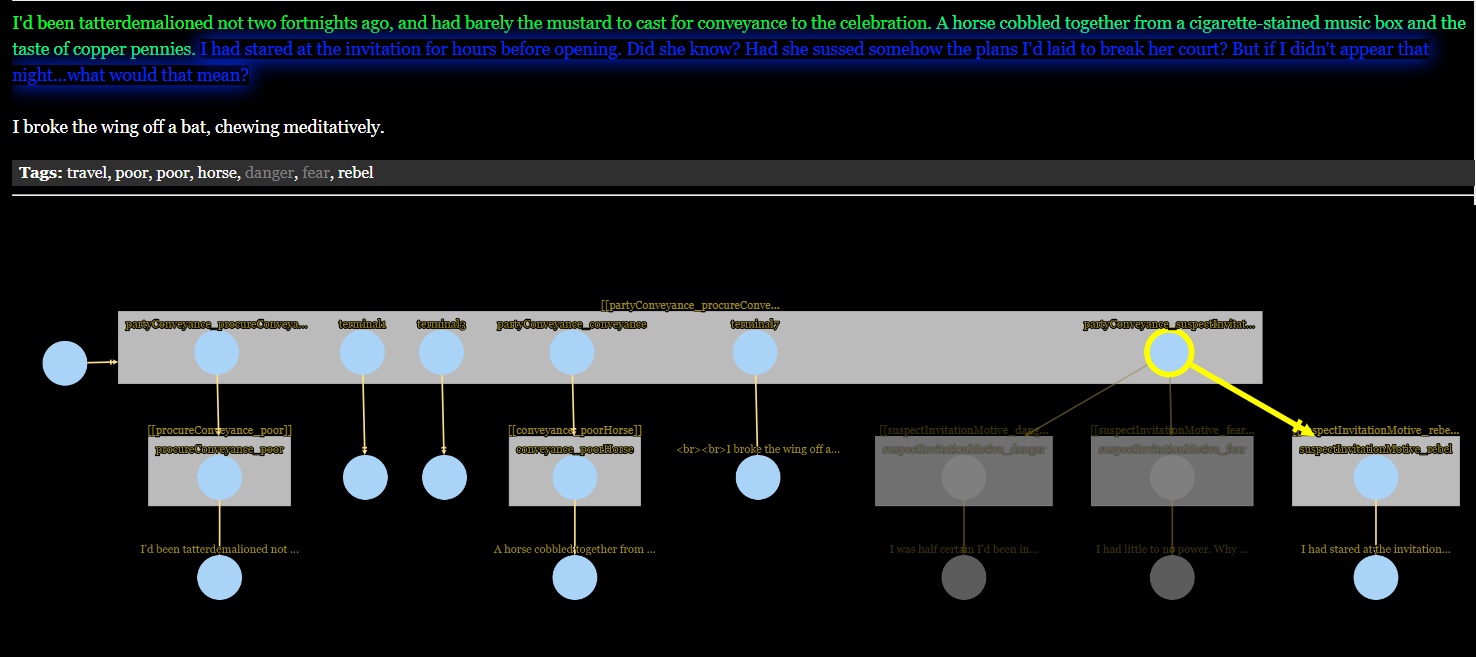
\includegraphics[width=\textwidth]{figures/4-Delve/memory-diagram.png}
    \caption{The memory surface text exploration tool. Here we can see the surface text (top) with the semantic tags beneath (travel, poor, poor, horse, etc) that are white if activated, and gray if not. In the bottom section, a graph shows the Expressionist grammar expansions. Right-clicking on a given section of text will highlight, on the graph, which expansion it corresponds to. Left-clicking will progress through the expansions cyclically, showing which semantic tags are activated in turn.}
    \label{fig:memory-diagram}
\end{figure}

%%%%%%%%%%%% END FIGURE %%%%%%%%%%%%%%%%%%%%%%%%%%%%%%%%

While still a prototype, and content authoring is still in its early stages, this visualization proved very useful in increasing Clarity for the authoring task of surface text. It was easy to quickly cycle between potential outputs, and immediately see what semantic tags would be activated. In future work, this would be integrated into the authoring tool, such that it would be easily accessible. Currently, it still requires exporting data from Expressionist's tool, then saving that in an appropriate directory before firing up the visualization.

\paragraph{Ontology Visualization}\label{par:delve-ontology-visualization}

An initial prototype was also made of an ontology visualization (Figure \ref{fig:ontology-viz}). A more evocative approach was taken with it, in order to explore potentially surfacing it to the player to let them control how generation occurred. The idea was that players could make alterations to the ontology, and see how those changes were reified in the content in-game. Cytoscape \cite{cytoscape} was again leveraged for interactive visualization, because it easily allowed the customization of such a graph, by easily dragging connections between nodes and then labeling them. 

%%%%%%%% BEGIN FIGURE %%%%%%%%%%%%%%%%%%%%%%%%%%%%%%%%%

\begin{figure}
    \centering
    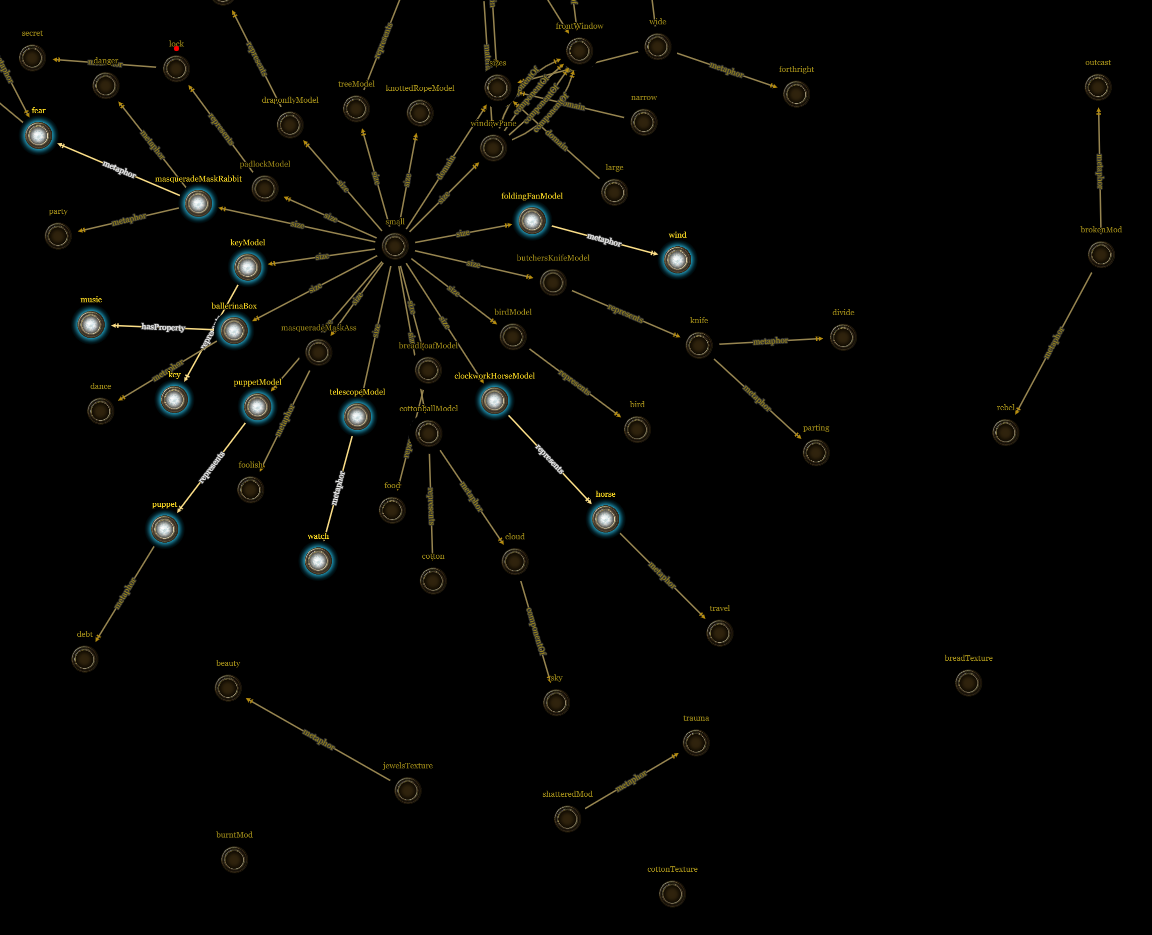
\includegraphics[width=\textwidth]{figures/4-Delve/substrate.png}
    \caption{A visualization of \textit{Delve}'s ontology, seen here with nodes highlighted for a given character's memories.}
    \label{fig:ontology-viz}
\end{figure}

%%%%%%%%%%%% END FIGURE %%%%%%%%%%%%%%%%%%%%%%%%%%%%%%%%

However, providing this capability proved wildly ambitious on the part of the designer, as it proved significantly difficult just for players to understand the relations in a static ontology being applied to content to make it dynamic, let alone allowing those relations to themselves be dynamic. While it was moderately useful to be able to see node data by right-clicking on it (Figure \ref{fig:substrate-detail}), there are less evocative, but more information-dense approaches for making ontology information explorable, such as those used by ConceptNet \cite{liu2004conceptnet}.

%%%%%%%% BEGIN FIGURE %%%%%%%%%%%%%%%%%%%%%%%%%%%%%%%%%

\begin{figure}
    \centering
    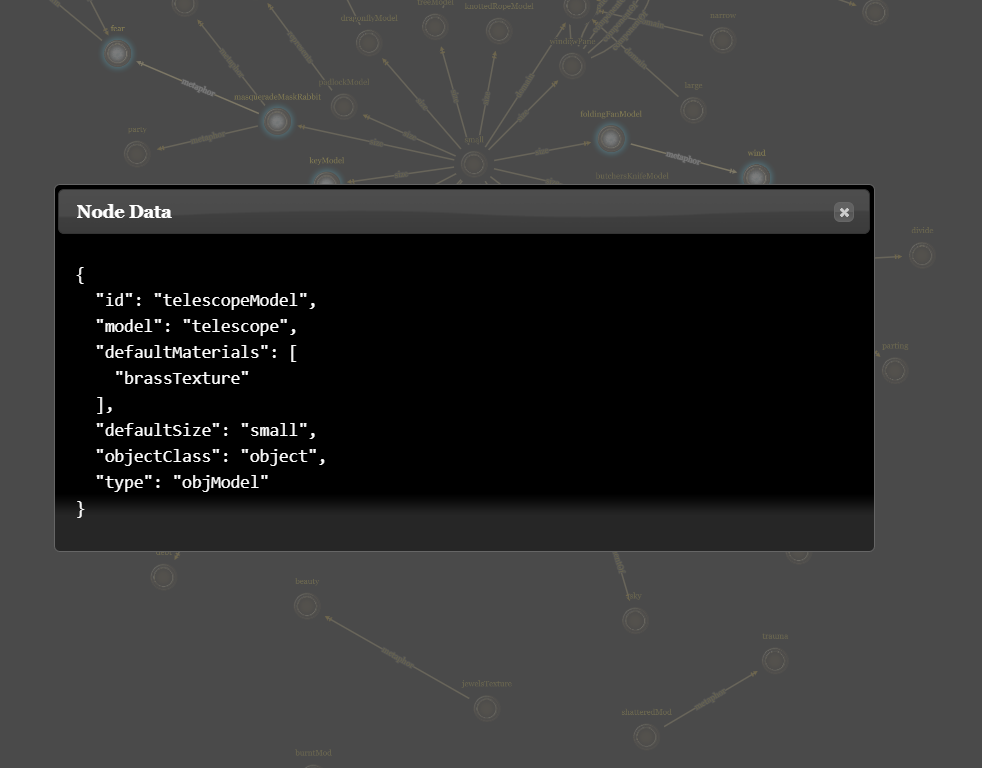
\includegraphics[width=\textwidth]{figures/4-Delve/substrate-detail.png}
    \caption{Right-clicking on a node in the ontology visualization brings up the node data for inspection.}
    \label{fig:substrate-detail}
\end{figure}

%%%%%%%%%%%% END FIGURE %%%%%%%%%%%%%%%%%%%%%%%%%%%%%%%%

\paragraph{Object Affordances}\label{par:delve-object-affordances}

Lastly, when authoring content we must also be mindful of the memory object affordances. This is currently not well-defined, which decreases Clarity significantly. For example: if we want to author a memory with a semantic tag of ``ice", and check to see how that is represented, and find out it could be realized as something made of glass, should we then look up to see what the metaphorical concept node is for ``broken", in case the player breaks it? Will that be an affordance? What if the object is put in a room with an ambient room asset, and the object is placed near it? Do we need to account for those potential concept nodes as well? As long as these questions are unanswered, it will decrease the Clarity for authoring, due to uncertainty in what tags may be required, and what we will need to author for, before we can consider a given surface text for a memory ``feature complete."

As mentioned in Section \ref{subsubsec:delve-writing-the-generative-grammars}, if it proves too narratively complex to have meaningful, plot-centric changes to memories bound to their semantic tags, we can also ``turn down the dial" on their impact, by relegating tag assignment to more non-critical variations, as with the shimmer text in \textit{Ice-Bound}. While this wouldn't necessarily increase our authorial Clarity as memories relate to objects, it would significantly lower the stakes for adding tags to a memory, although at the cost of making those changes seem less impactful, and thus cheapen the affordance.

Taking all these considerations together, we can see that currently we are at \textbf{Low Clarity}, though that may be raised, if the necessary tooling and visualization can be made to support authoring needs.

\subsubsection{Controllability}\label{subsubsec:delve-controllability}

The main interaction of \textit{Delve} centers around the manipulation of objects to affect memories. Therefore, we want to have as high a level of control around the relational output of the memory grammars as possible. It is a tall enough order to get the player to understand, for example, that cracks in an object's surface relate to fear. We could conceivably achieve this, as long as we reinforce the metaphorical connection across different memories, and allow the player to easily compare how the memory changes as they change the object. However, if (through lack of Controllability) that correspondence is not one-to-one, but instead is unpredictable, the task presented to the player becomes too difficult. Therefore, in terms of that correspondence, we want strict control over output.

However, in terms of coherency memory-to-memory, we can buy ourselves some leeway by leaning into the fiction of \textit{Delve} as a strange realm where many things may change. This could potentially lower the Contextuality, as we mentioned before, which in turn relaxes some of the Controllability requirements. However, despite that, in terms of thinking about the correspondence between text and object affordance, and the memories as they relate to each other through event generation, \textit{Delve}'s could be considered to have a \textbf{high Controllability} requirement.

\subsubsection{Authorability Summary}\label{subsubsec:delve-authorability-summary}

\textit{Delve} offers an intriguing and novel exploration of combinatorial content dynamics. Combining thematic combinatoric opportunities of \textit{Ice-Bound} with the recursive opportunities of StoryAssembler works could allow a uniquely expressive experience, once significant authoring has been done for it. However, even with some initial prototype tooling, we are still setting ourselves up for a challenge. While we are relying on our tried-and-true method of JSON data for most of the content authoring, the need for custom DSLs to drive the different dynamic effects gives us a \textbf{Medium Proficiency} requirement.

Authoring one ``unit" of content for \textit{Delve} also involves many different components, each with their own particular concerns and considerations. Because of this, it has a \textbf{High Complexity}, though that could potentially be reduced with the necessarily authoring tooling.

Lastly, current authoring for \textit{Delve} is at \textbf{Low Clarity}, though we have made some strides in increasing comprehensibility through visualizations. This is especially pernicious, given our need for \textbf{High Controllability}, though as mentioned in the Traversability summary, through potentially lowering Contextuality we could ameliorate that somewhat.

\section{Future Work}\label{sec:delve-future-work}

While \textit{Ice-Bound} and \textit{Emma's Journey} were finished before the Authoring Framework was formalized, \textit{Delve} provides an illustrative example of how to apply this framework to interrogate the authoring implications of generative narrative systems while content creation is just getting started, and highlight certain strategies we can take to make them more sustainable, and increase our authorial leverage.

From walking through each of these categories, we've reaffirmed that high Explorability and Replayability are core pillars of the experience, and thus will probably not easily be changed. We can make this easier to achieve incrementally, however, if we design content such that a single room can stand on its own to describe a character, and then move upward to two-character dynamics only after first establishing that feasibility. Thus, we can restrict ourselves to one-character events initially. Additionally, we can lower our Contextuality requirement, which proved so challenging in \textit{Emma's Journey}, if we instead adopt a more ``fires in the desert" approach, where each event can stand on its own, as opposed to focusing on more ``comb-like" structures which gain their expressive affordances by maintaining their contextuality over time. This could also increase the Reusability of content.

In terms of increasing our Authorability, we can put some initial effort into an authoring tool to unify the many different components required for one ``unit" of content, which should hopefully lower our Proficiency requirement, as well as Complexity. To push Complexity down a little further, we can also adopt an ``object-first" authoring method, such that our authoring stages are discretely divided up between ``object affordances" and ``memory representations of object affordances." This also would clear up some issues with Clarity, as it would provide us with a well-defined semantic tag requirement, which is easier to profile and write to, rather than the constant give-and-take of the method used for preliminary authoring tests.

\section{System Summary}\label{sec:delve-system-summary}

\textit{Delve} will prove a challenging experience to author for, though the expressive potential of the system is very promising. If successful, we will provide an experience with \textbf{High Explorability} and \textbf{High Replayability}, where players can manipulate objects to change the memories of characters. As long as we are conservative and careful with our authoring, we can get to \textbf{High Reusability} of our content, at the expense of dropping to \textbf{Low Contextuality} and keeping events more standalone.

In order to meet this challenge, we made the system such that we can author most content in JSON, as with previous systems. This in turn necessitated the use of DSLs, which gives us a \textbf{Medium Proficiency} requirement. Because of the many different components involved in one ``unit" of content, we'll need to try to provide tooling to unify the authoring of them as much as possible, because currently it suffers from \textbf{High Complexity}. Last of all, authoring for \textit{Delve} is currently at \textbf{Low Clarity} due to the difficulty in keeping the different dynamics straight while authoring the different components, though we have made some initial progress in alleviating that with visualization, as well as the plans outlined in Future Work (Section \ref{sec:delve-future-work}).